% Relatório de Palinologia e Mineração de Dados — Cololobus (Asteraceae)
% Template Springer Nature (sn-jnl)
% Versão complementada com as seções de Mineração de Dados e Aprendizado de Máquina.

\documentclass[pdflatex,sn-mathphys-num]{sn-jnl}

\usepackage{graphicx}%
\usepackage{multirow}%
\usepackage{amsmath,amssymb,amsfonts}%
\usepackage{amsthm}%
\usepackage{mathrsfs}%
\usepackage[title]{appendix}%
\usepackage{xcolor}%
\usepackage{textcomp}%
\usepackage{manyfoot}%
\usepackage{booktabs}%
\usepackage{float}%
\usepackage{placeins}%


\graphicspath{{../images/}{../images/prancha/}{../figuras/}}

\raggedbottom

\makeatletter
\patchcmd{\@maketitle}{Contributing authors:\ }{E-mail(s): }{}{}
\makeatother

\begin{document}

\title[Aprendizado de Máquina em morfologia polínica de \textit{Cololobus}]{Aplicação de Aprendizado de Máquina em morfologia polínica de \textit{Cololobus} H. Rob (\textit{Asteraceae}, Vernonieae)}

\author[1]{\fnm{Hugo} \sur{Sanchez de Sousa}}\email{hugo.sousa@ufu.br}




\affil[1]{\orgdiv{Instituto de Biologia, Programa de Pós-Graduação em Biologia Vegetal}, \orgname{Universidade Federal de Uberlândia}, \orgaddress{\city{Uberlândia}, \state{Minas Gerais}, \country{Brasil}}}

\abstract{Este estudo descreve a morfologia polínica de quatro espécies congêneres de \textit{Cololobus} endêmicas do Espírito Santo, combinando microscopia eletrônica de varredura, microscopia óptica e análise morfométrica quantitativa em vista equatorial. Os grãos são isopolares, oblato-esferoidais e 3-colporados, com exina equinada-microperfurada. Medidas de eixo polar e equatorial, espessura da exina e dimensões dos espinhos diferem entre táxons, embora espécies congêneres apresentem sobreposição distribucional em diversas \textit{traits}. A análise exploratória confirma diferenças estatisticamente significativas em 11 de 14 variáveis morfométricas, destacando \textit{C. hatschbachii} como a espécie morfologicamente mais distinta. Como etapa de mineração de dados, aplicou-se classificação supervisionada das espécies a partir das 14 \textit{features} morfométricas: o melhor modelo (\textit{Support Vector Machine} com \textit{kernel} RBF, hiperparâmetros ajustados por busca em grade) alcançou F1-macro de $0{,}72$ em validação cruzada estratificada, muito acima da linha de base aleatória ($0{,}21$). \textit{C. hatschbachii} foi a espécie mais bem classificada, enquanto \textit{C. longiangustatus}, \textit{C. rupestris} e \textit{C. ruschianus} concentram os erros, corroborando a forte sobreposição morfométrica observada na análise exploratória.}

\keywords{\textit{Cololobus}, palinologia, Asteraceae, Vernonieae, morfometria, mineração de dados, aprendizado de máquina}

\maketitle

%%======================================================================
\section{Introdução}\label{sec:introducao}
%%======================================================================

Asteraceae Bercht. \& J. Presl constitui uma das maiores famílias de Angiospermas, sendo considerada uma das mais distintas e naturais entre as plantas com flores \cite{roque2017}. Compreende mais de 1.600 gêneros e aproximadamente 24.000 espécies distribuídas em todos os continentes, apresentando maior diversidade em regiões temperadas e semiáridas dos trópicos e subtrópicos \cite{funk2009}. A ampla distribuição geográfica, associada à elevada riqueza específica e diversidade morfológica, torna a família um dos grupos mais relevantes para estudos taxonômicos, sistemáticos e evolutivos.

Entre as tribos reconhecidas em Asteraceae, Vernonieae destaca-se pela expressiva diversidade de espécies e pela complexidade taxonômica de seus representantes. Atualmente, a tribo compreende cerca de 126 gêneros, 1.300 espécies e 21 subtribos \cite{robinson2007,keeley2009}. Entre as características diagnósticas de Vernonieae, destacam-se aspectos morfológicos e palinológicos amplamente utilizados na delimitação de seus táxons. Os grãos de pólen são predominantemente triaperturados e apresentam padrões de ornamentação característicos, geralmente do tipo equinolofado ou subequinolofado, constituindo importantes caracteres para estudos sistemáticos da tribo \cite{jones1979,esteves2017}.

Inserido em Vernonieae, \textit{Cololobus} H. Rob. é um gênero endêmico do estado do Espírito Santo, Brasil, atualmente composto por cinco espécies \cite{brito2022}. O gênero foi estabelecido por Robinson \cite{robinson1994} a partir das espécies \textit{Cololobus rupestris} H. Rob., \textit{Cololobus longiangustatus} (G.M. Barroso) H. Rob. e \textit{Cololobus hatschbachii} H. Rob., esta última designada como espécie-tipo. Posteriormente, \textit{Cololobus argenteus} M. Monge \& Semir e \textit{Cololobus ruschianus} M. Monge, Fraga \& A.P. Fontana foram descritas, ampliando o conhecimento sobre a diversidade e distribuição do grupo \cite{monge2018,monge2021,brito2022}. As espécies do gênero caracterizam-se pelo hábito subarbustivo, capítulos com seis séries de brácteas involucrais e corolas glabras com lobos fortemente reduzidos \cite{robinson2007}.

A palinologia tem desempenhado papel fundamental na sistemática vegetal, fornecendo caracteres morfológicos frequentemente informativos para a delimitação de táxons em diferentes níveis hierárquicos. Características como tamanho, forma, simetria, número e tipo de aberturas, além dos padrões de ornamentação da exina, constituem importantes fontes de evidência para estudos taxonômicos, filogenéticos e evolutivos. Em Asteraceae, os caracteres polínicos têm sido amplamente utilizados na circunscrição de gêneros, tribos e subtribos, contribuindo para o entendimento das relações evolutivas dentro da família \cite{skvarla1977,jones1979}. Além disso, os estudos palinológicos fornecem informações relevantes para investigações relacionadas à biologia reprodutiva, ecologia da polinização, biogeografia e conservação da biodiversidade.

Embora avanços significativos tenham sido obtidos no conhecimento taxonômico de \textit{Cololobus} nas últimas décadas, informações sobre a morfologia polínica de suas espécies permanecem escassas. Considerando a importância dos caracteres polínicos para a sistemática de Vernonieae, a caracterização dos grãos de pólen de \textit{Cololobus} pode fornecer evidências adicionais para a delimitação do gênero, espécies e subtribos, e para a compreensão de suas relações com outros grupos da tribo. Além da descrição qualitativa e da análise exploratória, o presente estudo incorpora uma etapa de \textit{mineração de dados}: a partir das medidas morfométricas quantitativas, avalia-se em que medida técnicas de \textit{aprendizado de máquina} conseguem discriminar automaticamente as espécies e quais variáveis são mais informativas para essa separação. Nesse contexto, o trabalho tem como objetivo descrever a morfologia polínica das espécies de \textit{Cololobus} e testar a separabilidade morfométrica dos táxons por classificação supervisionada, ampliando o conhecimento palinológico e contribuindo para o entendimento sistemático do gênero.

%%======================================================================
\section{Metodologia}\label{sec:metodologia}
%%======================================================================

\subsection{Material estudado}\label{subsec:material}

Foram analisados grãos de pólen de quatro espécies de \textit{Cololobus}: \textit{C. hatschbachii}, \textit{C. longiangustatus}, \textit{C. rupestris} e \textit{C. ruschianus}. O material botânico foi obtido a partir de espécimes depositados em herbários, cujos vouchers estão listados na Tab.~\ref{tab:vouchers}.

\subsection{Obtenção e preparo do material polínico}\label{subsec:preparo}

A técnica de acetólise de Erdtman \cite{erdtman1960}, com adaptações de laboratório, foi empregada para remover o conteúdo citoplasmático e a intina dos grãos de pólen, permitindo a visualização da exina. Inicialmente, capítulos de material de herbário foram fervidos em água destilada com gotas de detergente por cinco minutos, até a maceração das anteras. Com auxílio de estereomicroscópio, as anteras foram abertas em placa de Petri, com cuidado para separar os grãos de pólen dos demais tecidos vegetais. Os grãos foram transferidos para tubos de ensaio, lavados com água destilada e centrifugados (5~min), repetindo-se a lavagem até a eliminação de resíduos.

Na sequência, os grãos foram tratados com ácido acético glacial e centrifugados (5~min), descartando-se o sobrenadante em recipiente adequado na capela de exaustão; o procedimento foi repetido. Preparou-se então a solução acetolítica na proporção de nove partes de anidrido acético para uma parte de ácido sulfúrico (9:1). A solução acetolítica foi adicionada aos tubos (aproximadamente um terço do volume), homogeneizada com bastão de vidro e submetida a banho-maria a 80~$^{\circ}$C por 5~min, até o escurecimento da solução. Após resfriamento, os tubos foram centrifugados (3~min), o sobrenadante descartado e o material lavado com ácido acético e, em seguida, com água destilada, com centrifugações intermediárias de 5~min.

Como etapa de reidratação, os grãos permaneceram em água glicerinada (50\%) por 30~min, recuperando forma e tamanho. Após lavagem final com água destilada e centrifugação, os tubos foram mantidos de boca para baixo em estufa até a evaporação completa da umidade. O sucesso da acetólise foi verificado pela alteração da coloração dos grãos de amarelo/laranjado para marrom.

\subsection{Microscopia óptica}\label{subsec:mo}

Parte do material acetolizado foi montada em lâminas permanentes com gelatina glicerinada, derretida em placa aquecedora, e coberta com lâmínula selada com esmalte incolor. As lâminas foram preferencialmente preparadas no dia da acetólise. As observações em microscopia óptica compreenderam vistas equatorial e polar, registradas fotograficamente para composição da prancha morfológica (Fig.~\ref{fig:prancha}).

\subsection{Microscopia eletrônica de varredura}\label{subsec:mev}

Grãos de pólen acetolizados destinados à microscopia eletrônica de varredura (MEV) foram conservados em álcool 70\% a 4~$^{\circ}$C em tubos bem fechados, com adição de cristais de fenol para inibir proliferação fúngica. Para montagem nos \textit{stubs}, o material foi lavado duas vezes em álcool 96\% e uma vez em álcool absoluto, com centrifugação de 3~min entre cada etapa. Após eliminação do sobrenadante na última lavagem, os grãos foram depositados sobre os \textit{stubs}, metalizados com ouro e observados em microscópio eletrônico de varredura.

\subsection{Análise morfométrica}\label{subsec:morfometria}

Medidas quantitativas dos grãos em vista equatorial foram obtidas manualmente no software Fiji/ImageJ. Foram registradas 14 variáveis morfométricas, incluindo eixos polar e equatorial, área, perímetro, Feret, circularidade, solidez, dimensões das aberturas (ectoabertura e endoabertura), espessura da exina e dimensões dos espinhos. Apenas registros validados (\texttt{valid=1}) foram incluídos na análise. A exploração dos dados compreendeu: (i) avaliação de valores ausentes e \textit{outliers}; (ii) estatística descritiva e visualizações univariadas (histogramas, box plots e violin plots); (iii) testes de normalidade (Shapiro--Wilk) e de diferença entre espécies (Kruskal--Wallis, $\alpha = 0{,}05$); (iv) matriz de correlação entre \textit{features}; (v) análise de componentes principais (PCA) sobre dados padronizados (\textit{z-score}); e (vi) gráficos de dispersão bivariados e perfil morfométrico por espécie.

\subsection{Mineração de dados e aprendizado de máquina}\label{subsec:mineracao}

A etapa quantitativa foi estruturada como um problema de mineração de dados a partir de um conjunto tabular de 89 grãos válidos (\texttt{valid=1}), cada um descrito pelas 14 \textit{features} morfométricas (Tab.~\ref{tab:features}). O rótulo de classe corresponde à espécie (\texttt{species}), configurando uma tarefa de \textbf{classificação supervisionada} multiclasse com quatro classes aproximadamente balanceadas (21--24 grãos por espécie).

\paragraph{Pré-processamento.} O fluxo consistiu em: (i) exclusão de registros inválidos (\texttt{valid=0}); (ii) conversão de células vazias e do marcador \texttt{NI} em valores ausentes; (iii) imputação da mediana por vista para as variáveis com dados faltantes --- estratégia relevante porque as medidas de abertura concentram de 34\% a 48\% de ausências (Tab.~\ref{tab:features}); e (iv) padronização (\textit{z-score}, \texttt{StandardScaler}) das variáveis numéricas, necessária para modelos sensíveis à escala. \textit{Outliers} foram identificados pela regra do intervalo interquartílico (IQR $1{,}5\times$) e mantidos, por representarem variabilidade biológica legítima em amostra pequena.

\paragraph{Algoritmos e justificativa.} Foram comparados três classificadores: um \textit{DummyClassifier} estratificado (linha de base), \textbf{Random Forest} e \textbf{\textit{Support Vector Machine}} (SVM) com \textit{kernel} RBF. O Random Forest foi escolhido por sua  capacidade de generalização com poucas amostras e variáveis correlacionadas, além de fornecer medidas de importância de variáveis diretamente interpretáveis do ponto de vista palinológico. O SVM RBF foi escolhido por modelar fronteiras de decisão não lineares em espaço de baixa dimensão, adequado a classes que se sobrepõem morfometricamente. Optou-se por não empregar \textit{deep learning}: com cerca de 22 grãos por espécie, redes profundas tenderiam ao \textit{overfitting} e não preservariam a interpretabilidade das medidas em $\mu$m exigida pela morfometria.

\paragraph{Ajuste de hiperparâmetros e validação.} Os hiperparâmetros foram otimizados por busca exaustiva em grade (\texttt{GridSearchCV}) com F1-macro como critério. Para o Random Forest variaram-se \texttt{n\_estimators} $\in \{100, 200, 300\}$, \texttt{max\_depth} $\in \{\text{None}, 5, 10, 15\}$, \texttt{min\_samples\_leaf} $\in \{1, 2, 4\}$ e \texttt{max\_features} $\in \{\text{sqrt}, \text{log2}\}$; para o SVM, $C \in \{0{,}1, 1, 10, 100\}$ e $\gamma \in \{\text{scale}, \text{auto}, 0{,}01, 0{,}1\}$. O desempenho foi estimado por validação cruzada estratificada de cinco \textit{folds}, preservando a proporção de classes. Adotou-se o F1-macro como métrica principal por tratar as classes de forma equilibrada, e a matriz de confusão foi construída com predições \textit{out-of-fold}. A importância das variáveis no modelo final foi avaliada por permutação. De forma complementar, aplicou-se a clusterização não supervisionada \textbf{K-Means} ($k=4$), comparando os agrupamentos aos rótulos verdadeiros pelo \textit{Adjusted Rand Index} (ARI), para verificar se a estrutura morfométrica separa as espécies sem uso de rótulos. As análises foram implementadas em Python com \texttt{scikit-learn} \cite{pedregosa2011}; o código-fonte acompanha esta entrega.

\subsection{Terminologia palinológica}\label{subsec:terminologia}

A terminologia adotada para descrever tamanho, tipo e demais características morfológicas dos grãos de pólen analisados foi baseada em Erdtman \cite{erdtman1952}, Keeley e Jones \cite{keeley1977,keeley1979} e Punt et al. \cite{punt2007}.

%%======================================================================
\section{Resultados}\label{sec:resultados}
%%======================================================================

\subsection{Morfologia}\label{subsec:morfologia}

As características micromorfológicas e as medidas dos grãos de pólen analisados são apresentadas na Fig.~\ref{fig:prancha} e na Tab.~\ref{tab:medidas}.

Os grãos de pólen das espécies de \textit{Cololobus} são médios, isopolares, com forma oblato-esferoidal ($P/E = 0{,}90$--$0{,}94$) (Fig.~\ref{fig:prancha}A--L; Tab.~\ref{tab:medidas}) e âmbito subcircular (Fig.~\ref{fig:prancha}B, E, H, K). São 3-colporados, com colpos longos e estreitos (Fig.~\ref{fig:prancha}A, D, G, J). A endoabertura é lalongada, apresentando constrição mediana (Fig.~\ref{fig:prancha}A, J). A exina apresenta espessura semelhante em \textit{C. hatschbachii}, \textit{C. longiangustatus} e \textit{C. ruschianus}, sendo mais delgada em \textit{C. rupestris} (Tab.~\ref{tab:medidas}). A ornamentação da exina é subequinolofada, com teto densamente microperfurado possuindo espinhos de base alargada e ápice agudo. Os espinhos são mais longos em \textit{C. hatschbachii} e \textit{C. longiangustatus} e mais curtos em \textit{C. rupestris} e \textit{C. ruschianus} (Fig.~\ref{fig:prancha}A--L; Tab.~\ref{tab:medidas}). De acordo com a classificação de Keeley e Jones \cite{keeley1977,keeley1979}, todos os grãos de pólen das espécies estudadas pertencem ao tipo~A.

\begin{table}[htbp]
\caption{Lista de espécies de \textit{Cololobus} e seus respectivos vouchers.}\label{tab:vouchers}
\small
\begin{tabular*}{\textwidth}{@{\extracolsep\fill}p{0.32\textwidth}p{0.62\textwidth}@{}}
\toprule
Espécie & Voucher \\
\midrule
\textit{C. hatschbachii} H.Rob. & P. Renon et al. 978 (HUFU) \\
\textit{C. longiangustatus} (G.M.Barroso) H.Rob. & T. S. Lorencini et al. 183 (UEC) \\
\textit{C. rupestris} (Gardner) H.Rob. & P. Renon et al. 942 (HUFU); M.A. Moraes \& B. Benevenuto 44 (HUFU) \\
\textit{C. ruschianus} M.Monge, Fraga \& A.P.Fontana & L. Kollman \& R. M. Pizziolo 11987 (HUFU); V. Demuner et al. 1340 \\
\botrule
\end{tabular*}
\end{table}

\begin{sidewaystable}[htbp]
\caption{Medidas e características dos grãos de pólen de \textit{Cololobus}. $P$ --- eixo polar; $E$ --- diâmetro do eixo equatorial; $P/E$ --- razão entre eixo polar e equatorial. As medidas de $P$, $E$, $P/E$, espessura da exina, comprimento e largura dos espinhos estão em $\mu$m (mínimo(média)máximo).}\label{tab:medidas}
\small
\begin{tabular*}{\textheight}{@{\extracolsep\fill}lccccccc@{}}
\toprule
Espécie & $P$ & $E$ & $P/E$ & Formato & Espessura exina & Comp. espinhos & Larg. espinhos \\
\midrule
\textit{C. hatschbachii} & 25{,}22(30{,}02)35{,}04 & 29{,}20(33{,}26)35{,}81 & 0{,}90 & Oblato-esferoidal & 1{,}37(2{,}58)3{,}47 & 2{,}61(4{,}15)6{,}09 & 0{,}92(1{,}36)1{,}87 \\
\textit{C. longiangustatus} & 30{,}22(32{,}82)35{,}63 & 32{,}86(34{,}55)37{,}32 & 0{,}94 & Oblato-esferoidal & 1{,}30(2{,}42)3{,}40 & 4{,}26(4{,}83)6{,}41 & 0{,}83(1{,}64)2{,}37 \\
\textit{C. rupestris} & 29{,}01(31{,}65)33{,}81 & 30{,}16(34{,}08)38{,}18 & 0{,}92 & Oblato-esferoidal & 1{,}40(1{,}81)2{,}28 & 3{,}77(3{,}18)6{,}80 & 1{,}07(1{,}64)2{,}99 \\
\textit{C. ruschianus} & 30{,}31(32{,}99)36{,}34 & 32{,}62(34{,}89)37{,}87 & 0{,}94 & Oblato-esferoidal & 1{,}56(2{,}58)3{,}30 & 2{,}86(3{,}79)5{,}24 & 0{,}96(1{,}46)2{,}20 \\
\botrule
\end{tabular*}
\end{sidewaystable}

% Tabela gerada por scripts/generate_latex_morpho_table.py
% Inclua no relatório com: % Tabela gerada por scripts/generate_latex_morpho_table.py
% Inclua no relatório com: % Tabela gerada por scripts/generate_latex_morpho_table.py
% Inclua no relatório com: \input{tabela_cololobus_morfometria.tex}
% Requer no preâmbulo: \usepackage{booktabs}, \usepackage{multirow}

\begin{sidewaystable}[htbp]
\caption{Dados quantitativos dos grãos de pólen de espécies de \textit{Cololobus} (Asteraceae) em vista equatorial: diâmetro polar e equatorial ($\mu$m).}
\label{tab:cololobus_morfometria}
\begin{tabular*}{\textheight}{@{\extracolsep\fill}lcccccccc}
\toprule
& \multicolumn{4}{@{}c@{}}{Diâmetro polar em vista equatorial} & \multicolumn{4}{@{}c@{}}{Diâmetro equatorial em vista equatorial} \\
\cmidrule{2-5}\cmidrule{6-9}
Espécie & (R) $\bar{x} \pm S_{\bar{x}}$ & $S$ & IC & $V$ & (R) $\bar{x} \pm S_{\bar{x}}$ & $S$ & IC & $V$ \\
\midrule
\textit{C. hatschbachi}$^{*}$ & (25.22--35.05) $30.02 \pm 2.16$ & 0.46 & 29.06--30.98 & 7.20 & (29.20--35.82) $33.22 \pm 1.71$ & 0.36 & 32.46--33.98 & 5.15 \\
\textit{C. longiangustatus}$^{*}$ & (30.22--35.63) $32.83 \pm 1.34$ & 0.27 & 32.26--33.39 & 4.09 & (30.93--37.33) $34.56 \pm 1.52$ & 0.31 & 33.92--35.20 & 4.39 \\
\textit{C. rupestris}$^{*}$ & (29.01--33.82) $31.66 \pm 1.31$ & 0.29 & 31.06--32.25 & 4.13 & (30.17--38.19) $34.08 \pm 2.05$ & 0.45 & 33.15--35.02 & 6.01 \\
\textit{C. ruschianur}$^{*}$ & (30.31--36.34) $32.99 \pm 1.85$ & 0.40 & 32.15--33.83 & 5.62 & (32.63--37.88) $34.89 \pm 1.43$ & 0.31 & 34.24--35.55 & 4.10 \\
\botrule
\end{tabular*}
\footnotetext{$R$ = amplitude (mín.--máx.); $\bar{x}$ = média ($\mu$m); $S_{\bar{x}}$ = desvio padrão ($\mu$m); $S$ = erro padrão da média ($\mu$m); IC = intervalo de confiança de 95\% ($\mu$m); $V$ = coeficiente de variação (\%); $^{*}$\,$n < 25$; $^{**}$\,$n = 1$. Medidas obtidas no Fiji/ImageJ; apenas registros com \texttt{valid=1}.}
\end{sidewaystable}

% Requer no preâmbulo: \usepackage{booktabs}, \usepackage{multirow}

\begin{sidewaystable}[htbp]
\caption{Dados quantitativos dos grãos de pólen de espécies de \textit{Cololobus} (Asteraceae) em vista equatorial: diâmetro polar e equatorial ($\mu$m).}
\label{tab:cololobus_morfometria}
\begin{tabular*}{\textheight}{@{\extracolsep\fill}lcccccccc}
\toprule
& \multicolumn{4}{@{}c@{}}{Diâmetro polar em vista equatorial} & \multicolumn{4}{@{}c@{}}{Diâmetro equatorial em vista equatorial} \\
\cmidrule{2-5}\cmidrule{6-9}
Espécie & (R) $\bar{x} \pm S_{\bar{x}}$ & $S$ & IC & $V$ & (R) $\bar{x} \pm S_{\bar{x}}$ & $S$ & IC & $V$ \\
\midrule
\textit{C. hatschbachi}$^{*}$ & (25.22--35.05) $30.02 \pm 2.16$ & 0.46 & 29.06--30.98 & 7.20 & (29.20--35.82) $33.22 \pm 1.71$ & 0.36 & 32.46--33.98 & 5.15 \\
\textit{C. longiangustatus}$^{*}$ & (30.22--35.63) $32.83 \pm 1.34$ & 0.27 & 32.26--33.39 & 4.09 & (30.93--37.33) $34.56 \pm 1.52$ & 0.31 & 33.92--35.20 & 4.39 \\
\textit{C. rupestris}$^{*}$ & (29.01--33.82) $31.66 \pm 1.31$ & 0.29 & 31.06--32.25 & 4.13 & (30.17--38.19) $34.08 \pm 2.05$ & 0.45 & 33.15--35.02 & 6.01 \\
\textit{C. ruschianur}$^{*}$ & (30.31--36.34) $32.99 \pm 1.85$ & 0.40 & 32.15--33.83 & 5.62 & (32.63--37.88) $34.89 \pm 1.43$ & 0.31 & 34.24--35.55 & 4.10 \\
\botrule
\end{tabular*}
\footnotetext{$R$ = amplitude (mín.--máx.); $\bar{x}$ = média ($\mu$m); $S_{\bar{x}}$ = desvio padrão ($\mu$m); $S$ = erro padrão da média ($\mu$m); IC = intervalo de confiança de 95\% ($\mu$m); $V$ = coeficiente de variação (\%); $^{*}$\,$n < 25$; $^{**}$\,$n = 1$. Medidas obtidas no Fiji/ImageJ; apenas registros com \texttt{valid=1}.}
\end{sidewaystable}

% Requer no preâmbulo: \usepackage{booktabs}, \usepackage{multirow}

\begin{sidewaystable}[htbp]
\caption{Dados quantitativos dos grãos de pólen de espécies de \textit{Cololobus} (Asteraceae) em vista equatorial: diâmetro polar e equatorial ($\mu$m).}
\label{tab:cololobus_morfometria}
\begin{tabular*}{\textheight}{@{\extracolsep\fill}lcccccccc}
\toprule
& \multicolumn{4}{@{}c@{}}{Diâmetro polar em vista equatorial} & \multicolumn{4}{@{}c@{}}{Diâmetro equatorial em vista equatorial} \\
\cmidrule{2-5}\cmidrule{6-9}
Espécie & (R) $\bar{x} \pm S_{\bar{x}}$ & $S$ & IC & $V$ & (R) $\bar{x} \pm S_{\bar{x}}$ & $S$ & IC & $V$ \\
\midrule
\textit{C. hatschbachi}$^{*}$ & (25.22--35.05) $30.02 \pm 2.16$ & 0.46 & 29.06--30.98 & 7.20 & (29.20--35.82) $33.22 \pm 1.71$ & 0.36 & 32.46--33.98 & 5.15 \\
\textit{C. longiangustatus}$^{*}$ & (30.22--35.63) $32.83 \pm 1.34$ & 0.27 & 32.26--33.39 & 4.09 & (30.93--37.33) $34.56 \pm 1.52$ & 0.31 & 33.92--35.20 & 4.39 \\
\textit{C. rupestris}$^{*}$ & (29.01--33.82) $31.66 \pm 1.31$ & 0.29 & 31.06--32.25 & 4.13 & (30.17--38.19) $34.08 \pm 2.05$ & 0.45 & 33.15--35.02 & 6.01 \\
\textit{C. ruschianur}$^{*}$ & (30.31--36.34) $32.99 \pm 1.85$ & 0.40 & 32.15--33.83 & 5.62 & (32.63--37.88) $34.89 \pm 1.43$ & 0.31 & 34.24--35.55 & 4.10 \\
\botrule
\end{tabular*}
\footnotetext{$R$ = amplitude (mín.--máx.); $\bar{x}$ = média ($\mu$m); $S_{\bar{x}}$ = desvio padrão ($\mu$m); $S$ = erro padrão da média ($\mu$m); IC = intervalo de confiança de 95\% ($\mu$m); $V$ = coeficiente de variação (\%); $^{*}$\,$n < 25$; $^{**}$\,$n = 1$. Medidas obtidas no Fiji/ImageJ; apenas registros com \texttt{valid=1}.}
\end{sidewaystable}


\begin{figure}[H]
\centering
\includegraphics[width=0.98\textwidth,height=0.68\textheight,keepaspectratio]{Prancha_polen.png}
\caption{Grãos de pólen das espécies de \textit{Cololobus} em microscopia eletrônica de varredura e microscopia óptica. A--C. \textit{C. hatschbachii}; D--F. \textit{C. longiangustatus}; G--I. \textit{C. rupestris}; J--L. \textit{C. ruschianus}. A. Vista equatorial; observar endoabertura com constrição mediana e espinhos longos. B. Vista polar. C. Vista equatorial. D. Vista equatorial; observar colpo estreito e espinhos longos. E. Vista polar. F. Vista equatorial; observar colpo e endoabertura. G. Vista equatorial; observar espinhos curtos. H. Vista polar. I. Vista equatorial. J. Vista equatorial; observar endoabertura e espinhos curtos. K. Vista polar. L. Vista equatorial.}\label{fig:prancha}
\end{figure}

\subsection{Análise exploratória morfométrica}\label{subsec:eda}

A análise exploratória foi conduzida sobre 89 grãos válidos de quatro espécies, com 14 medidas morfométricas obtidas manualmente no Fiji/ImageJ em vista equatorial (Tab.~\ref{tab:features}).

\paragraph{Qualidade dos dados.} As medidas de abertura concentraram os maiores percentuais de valores ausentes (34--48\%; Fig.~\ref{fig:missing}), seguidas pela espessura da exina (29\%). Eixos polar e equatorial apresentaram menos de 2\% de ausências. A detecção de \textit{outliers} pela regra IQR ($1{,}5\times$) indicou maior frequência em variáveis de abertura e circularidade (Fig.~\ref{fig:outliers}); 59 grãos apresentaram pelo menos um valor atípico em alguma \textit{feature}, mas foram mantidos por representarem variabilidade biológica legítima.

\begin{figure}[H]
\centering
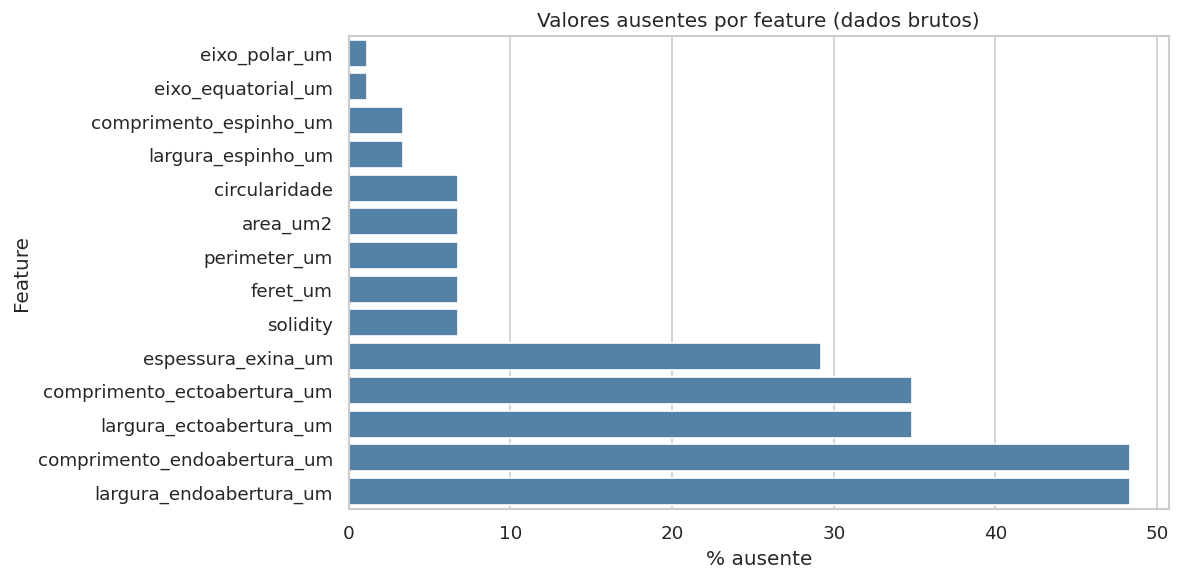
\includegraphics[width=0.85\textwidth]{missing_por_feature.png}
\caption{Percentual de valores ausentes por \textit{feature} morfométrica (antes da imputação).}\label{fig:missing}
\end{figure}

\begin{figure}[H]
\centering
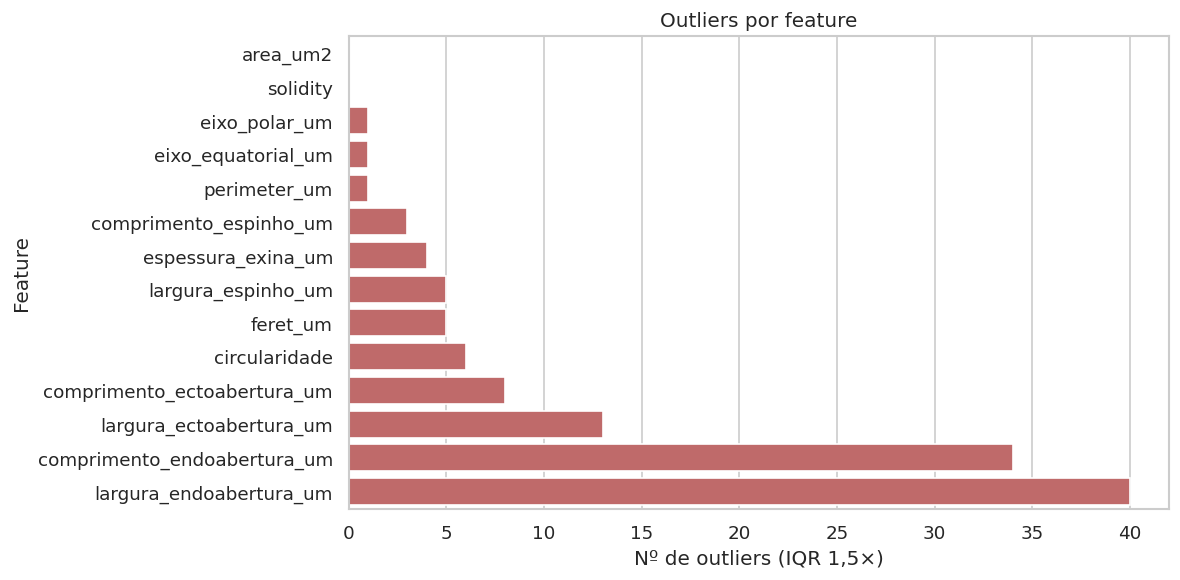
\includegraphics[width=0.85\textwidth]{outliers_por_feature.png}
\caption{Número de \textit{outliers} detectados por \textit{feature} (regra IQR $1{,}5\times$; dados imputados).}\label{fig:outliers}
\end{figure}

\paragraph{Distribuições univariadas.} Os histogramas (Fig.~\ref{fig:histogramas}) e os box plots (Fig.~\ref{fig:boxplots}) revelam assimetria e caudas longas em diversas variáveis, especialmente circularidade e medidas de abertura. Os violin plots (Fig.~\ref{fig:violinos}) confirmam que \textit{C. hatschbachii} apresenta menor área ($\approx$940~$\mu$m$^2$) e perímetro ($\approx$225~$\mu$m), além de maior solidez ($\approx$0,87), destacando-se como a espécie morfologicamente mais distinta. \textit{C. rupestris} tende a apresentar maior largura da ectoabertura ($\approx$7,3~$\mu$m), enquanto \textit{C. longiangustatus} e \textit{C. ruschianus} exibem perfis muito semelhantes em área, eixos e aberturas, com forte sobreposição distribucional.

\begin{figure}[H]
\centering
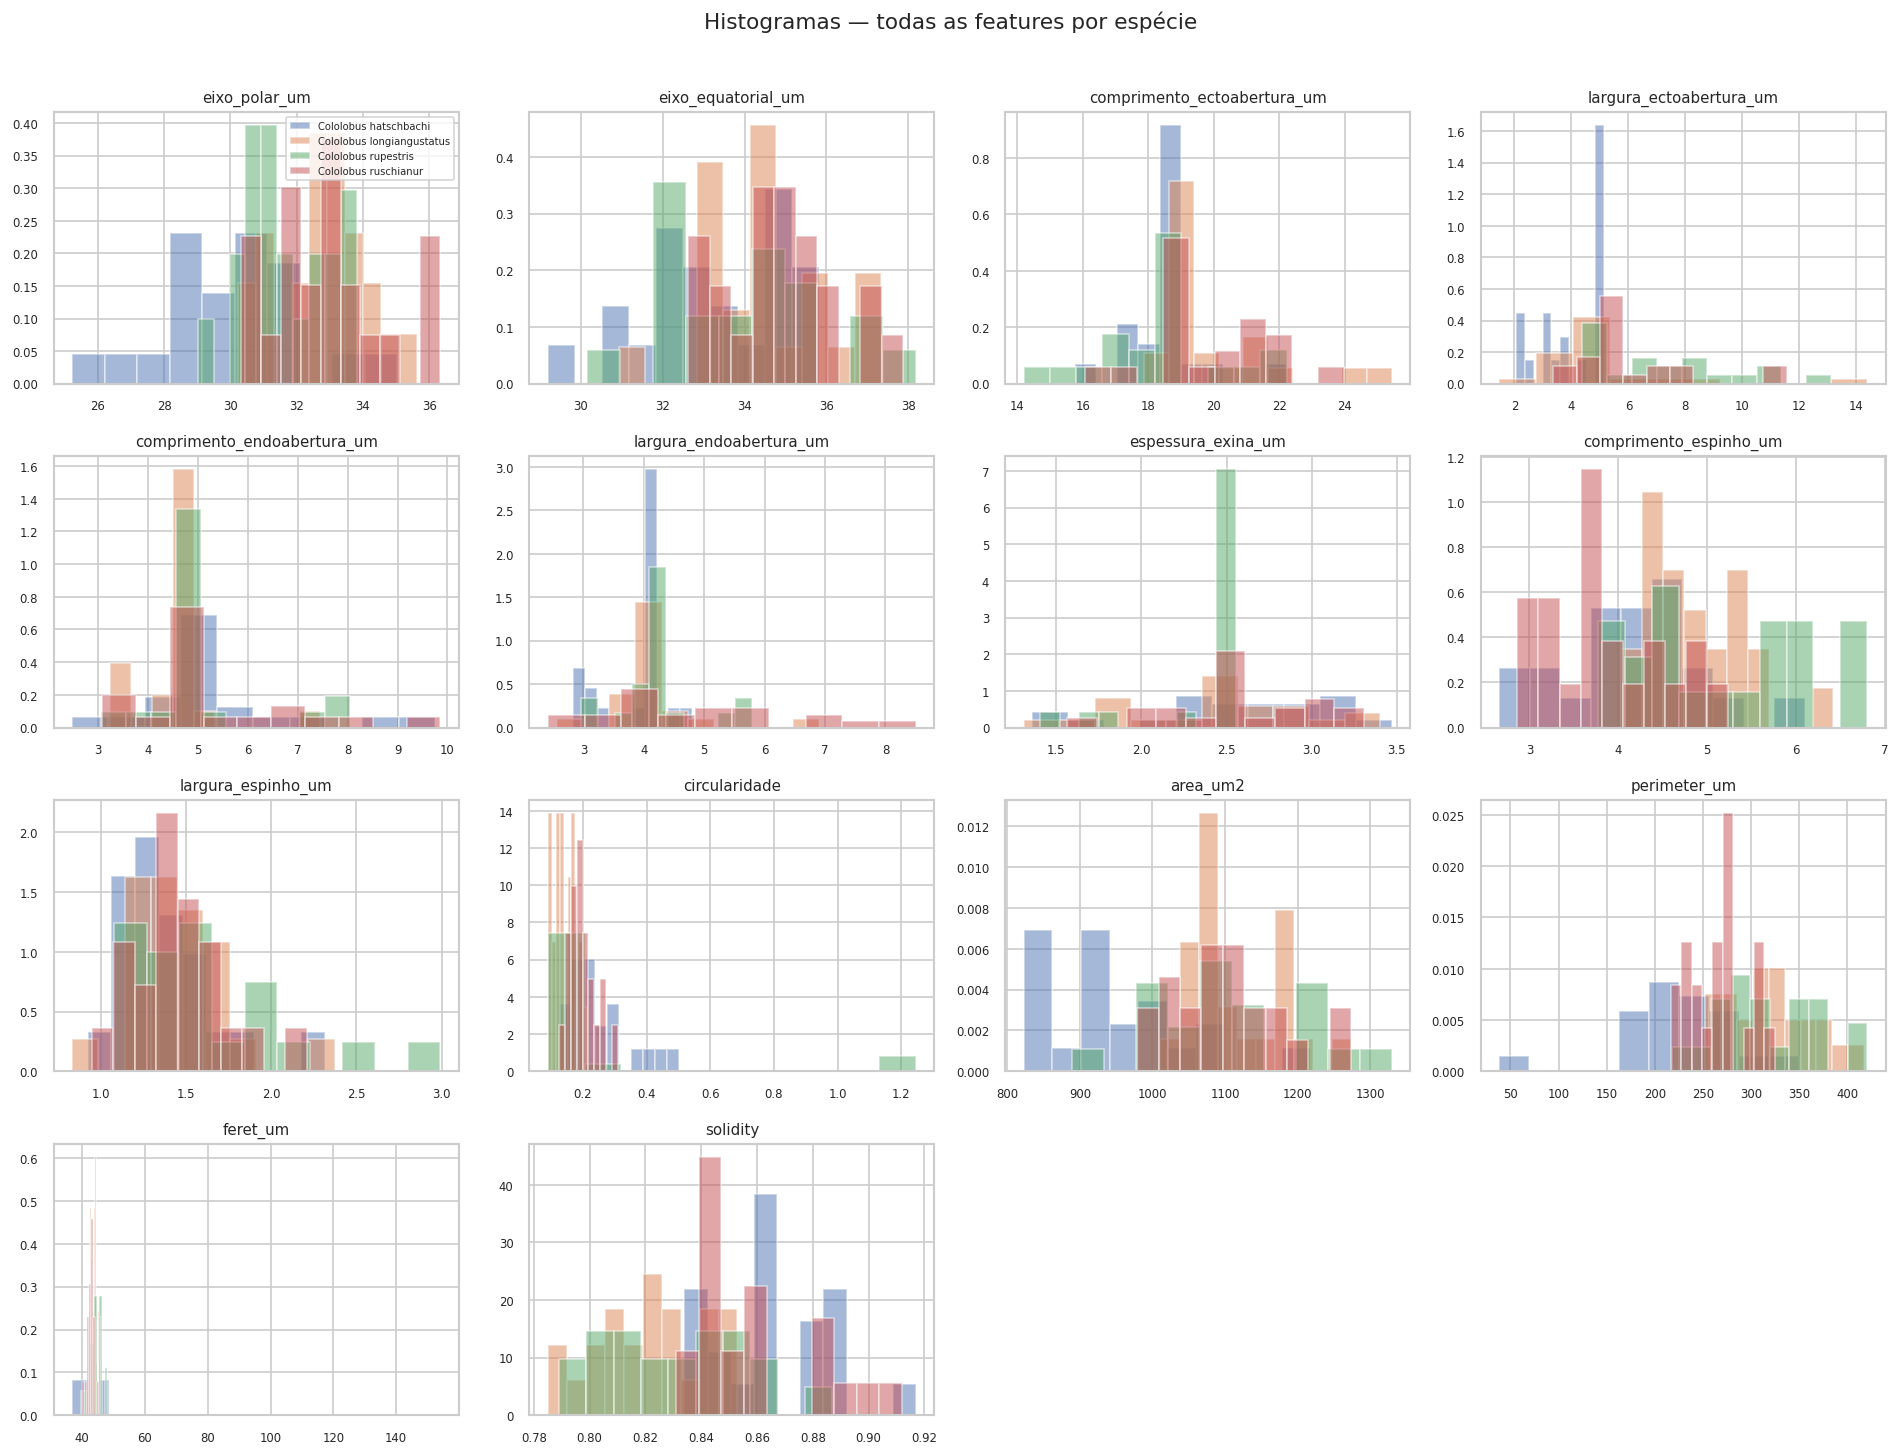
\includegraphics[width=0.98\textwidth,height=0.9\textheight,keepaspectratio]{histogramas_todas_features.png}
\caption{Histogramas das 14 \textit{features} morfométricas por espécie (escala original em $\mu$m ou adimensional).}\label{fig:histogramas}
\end{figure}

\begin{figure}[H]
\centering
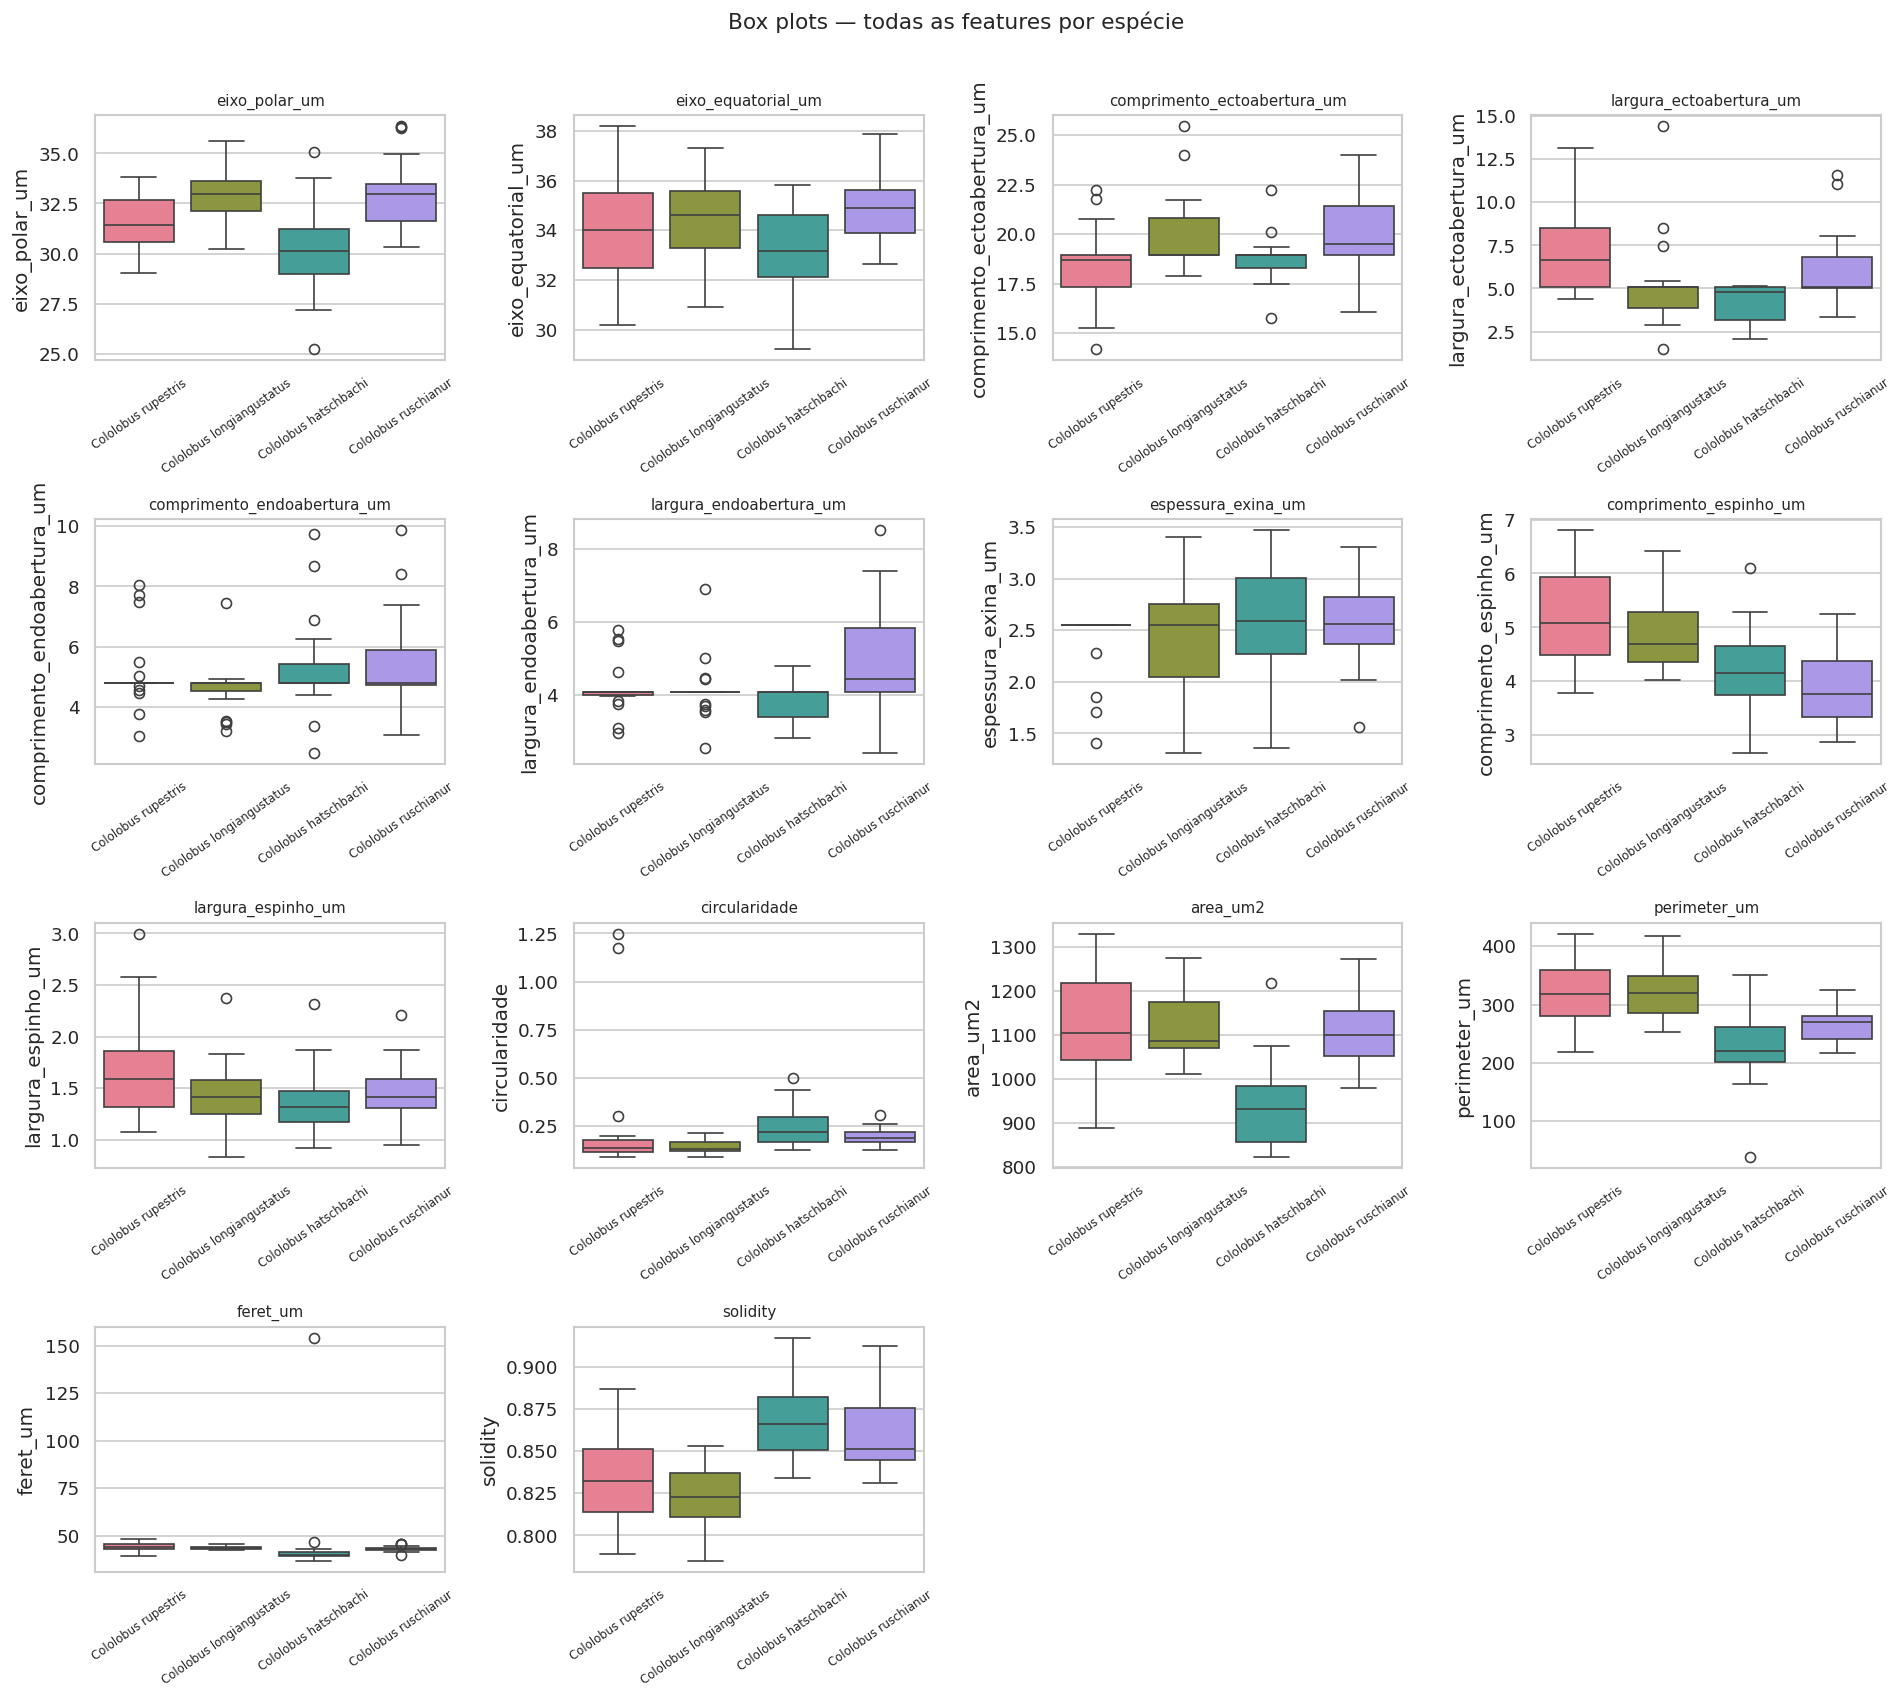
\includegraphics[width=0.98\textwidth,height=0.9\textheight,keepaspectratio]{boxplots_todas_features.png}
\caption{Box plots das 14 \textit{features} morfométricas por espécie. A linha central indica a mediana; os pontos representam grãos individuais.}\label{fig:boxplots}
\end{figure}

\begin{figure}[H]
\centering
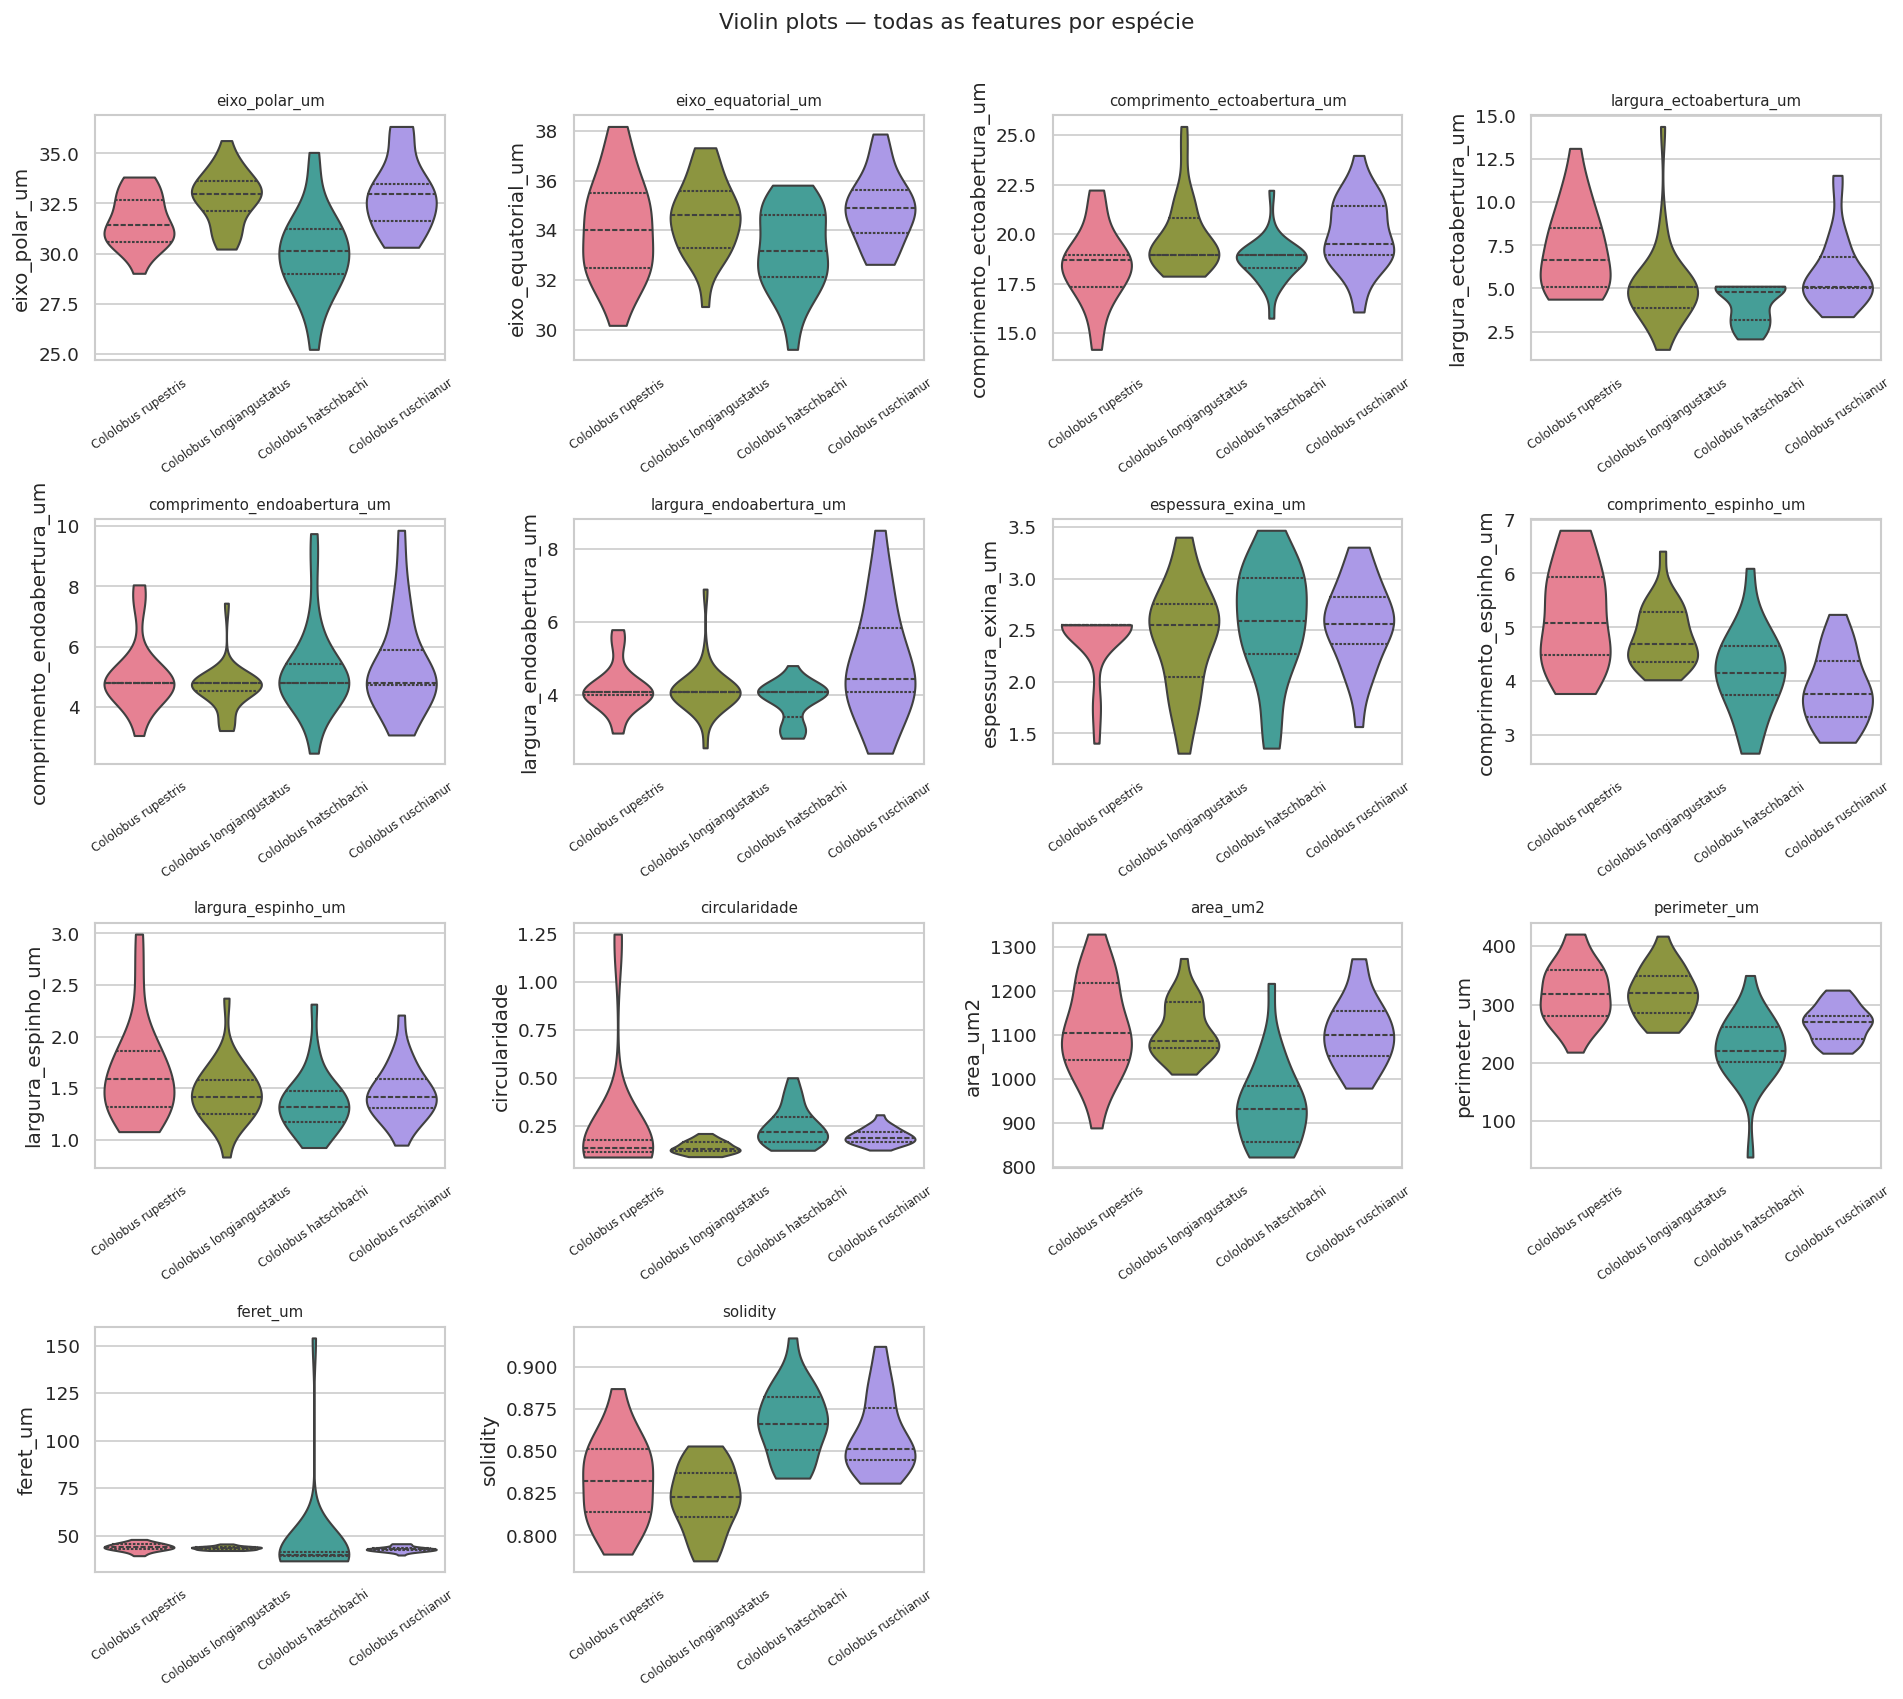
\includegraphics[width=0.98\textwidth,height=0.9\textheight,keepaspectratio]{violinos_todas_features.png}
\caption{Distribuição das 14 features morfométricas por espécie (violin plots). A linha central indica a mediana.}\label{fig:violinos}
\end{figure}

\paragraph{Normalidade e diferenças entre espécies.} O teste de Shapiro--Wilk ($\alpha = 0{,}05$) indicou compatibilidade com normalidade em apenas 5 das 14 variáveis na amostra global imputada (Fig.~\ref{fig:shapiro}), justificando o uso de métodos não paramétricos. O teste de Kruskal--Wallis revelou diferenças significativas entre espécies em 11 das 14 \textit{features} (Tab.~\ref{tab:features}; Fig.~\ref{fig:kruskal}). As variáveis mais discriminantes incluíram perímetro, solidez, área, Feret, comprimento do espinho, circularidade e eixo polar; não significativas foram largura do espinho, comprimento da endoabertura e espessura da exina.

% Tabela das 14 features morfométricas analisadas.
% Combina EDA (valores ausentes + Kruskal-Wallis) e ML (importância por permutação).
% Inclua no relatório com: % Tabela das 14 features morfométricas analisadas.
% Combina EDA (valores ausentes + Kruskal-Wallis) e ML (importância por permutação).
% Inclua no relatório com: % Tabela das 14 features morfométricas analisadas.
% Combina EDA (valores ausentes + Kruskal-Wallis) e ML (importância por permutação).
% Inclua no relatório com: \input{tabela_features_analisadas.tex}
% Requer no preâmbulo: \usepackage{booktabs}

\begin{table}[htbp]
\caption{Conjunto de 14 \textit{features} morfométricas analisadas. Percentual de valores ausentes (antes da imputação), estatística $H$ e $p$-valor do teste de Kruskal-Wallis para diferença entre espécies ($\alpha = 0{,}05$) e importância por permutação no modelo de classificação final (SVM RBF; F1-macro como métrica). Ordenado pela significância no Kruskal-Wallis.}\label{tab:features}
\small
\begin{tabular*}{\textwidth}{@{\extracolsep\fill}lccccc@{}}
\toprule
\textit{Feature} & Ausentes (\%) & $H$ & $p$-valor & Signif. & Imp.\ perm. \\
\midrule
Perímetro ($\mu$m)            & 6{,}7  & 39{,}88 & $1{,}1\times10^{-8}$ & sim & 0{,}026 \\
Solidez                        & 6{,}7  & 39{,}14 & $1{,}6\times10^{-8}$ & sim & 0{,}067 \\
Área ($\mu$m$^2$)              & 6{,}7  & 33{,}26 & $2{,}8\times10^{-7}$ & sim & 0{,}040 \\
Feret ($\mu$m)                 & 6{,}7  & 29{,}72 & $1{,}6\times10^{-6}$ & sim & --- \\
Comp.\ do espinho ($\mu$m)     & 3{,}4  & 29{,}47 & $1{,}8\times10^{-6}$ & sim & 0{,}092 \\
Circularidade                  & 6{,}7  & 28{,}72 & $2{,}6\times10^{-6}$ & sim & --- \\
Eixo polar ($\mu$m)            & 1{,}1  & 27{,}30 & $5{,}1\times10^{-6}$ & sim & 0{,}076 \\
Larg.\ ectoabertura ($\mu$m)   & 34{,}8 & 22{,}94 & $4{,}2\times10^{-5}$ & sim & 0{,}057 \\
Comp.\ ectoabertura ($\mu$m)   & 34{,}8 & 16{,}92 & $7{,}4\times10^{-4}$ & sim & 0{,}038 \\
Eixo equatorial ($\mu$m)       & 1{,}1  & 9{,}85  & $2{,}0\times10^{-2}$ & sim & --- \\
Larg.\ endoabertura ($\mu$m)   & 48{,}3 & 8{,}97  & $3{,}0\times10^{-2}$ & sim & 0{,}033 \\
Larg.\ do espinho ($\mu$m)     & 3{,}4  & 5{,}71  & $1{,}3\times10^{-1}$ & não & --- \\
Comp.\ endoabertura ($\mu$m)   & 48{,}3 & 3{,}57  & $3{,}1\times10^{-1}$ & não & 0{,}035 \\
Espessura da exina ($\mu$m)    & 29{,}2 & 3{,}12  & $3{,}7\times10^{-1}$ & não & 0{,}030 \\
\botrule
\end{tabular*}
\footnotetext{Signif. = diferença estatisticamente significativa entre espécies ($p < 0{,}05$). Imp.\ perm. = queda média em F1-macro ao permutar a variável; ``---'' indica variável fora do \textit{top} 10 de importância. Base: 89 grãos válidos (\texttt{valid=1}), vista equatorial.}
\end{table}

% Requer no preâmbulo: \usepackage{booktabs}

\begin{table}[htbp]
\caption{Conjunto de 14 \textit{features} morfométricas analisadas. Percentual de valores ausentes (antes da imputação), estatística $H$ e $p$-valor do teste de Kruskal-Wallis para diferença entre espécies ($\alpha = 0{,}05$) e importância por permutação no modelo de classificação final (SVM RBF; F1-macro como métrica). Ordenado pela significância no Kruskal-Wallis.}\label{tab:features}
\small
\begin{tabular*}{\textwidth}{@{\extracolsep\fill}lccccc@{}}
\toprule
\textit{Feature} & Ausentes (\%) & $H$ & $p$-valor & Signif. & Imp.\ perm. \\
\midrule
Perímetro ($\mu$m)            & 6{,}7  & 39{,}88 & $1{,}1\times10^{-8}$ & sim & 0{,}026 \\
Solidez                        & 6{,}7  & 39{,}14 & $1{,}6\times10^{-8}$ & sim & 0{,}067 \\
Área ($\mu$m$^2$)              & 6{,}7  & 33{,}26 & $2{,}8\times10^{-7}$ & sim & 0{,}040 \\
Feret ($\mu$m)                 & 6{,}7  & 29{,}72 & $1{,}6\times10^{-6}$ & sim & --- \\
Comp.\ do espinho ($\mu$m)     & 3{,}4  & 29{,}47 & $1{,}8\times10^{-6}$ & sim & 0{,}092 \\
Circularidade                  & 6{,}7  & 28{,}72 & $2{,}6\times10^{-6}$ & sim & --- \\
Eixo polar ($\mu$m)            & 1{,}1  & 27{,}30 & $5{,}1\times10^{-6}$ & sim & 0{,}076 \\
Larg.\ ectoabertura ($\mu$m)   & 34{,}8 & 22{,}94 & $4{,}2\times10^{-5}$ & sim & 0{,}057 \\
Comp.\ ectoabertura ($\mu$m)   & 34{,}8 & 16{,}92 & $7{,}4\times10^{-4}$ & sim & 0{,}038 \\
Eixo equatorial ($\mu$m)       & 1{,}1  & 9{,}85  & $2{,}0\times10^{-2}$ & sim & --- \\
Larg.\ endoabertura ($\mu$m)   & 48{,}3 & 8{,}97  & $3{,}0\times10^{-2}$ & sim & 0{,}033 \\
Larg.\ do espinho ($\mu$m)     & 3{,}4  & 5{,}71  & $1{,}3\times10^{-1}$ & não & --- \\
Comp.\ endoabertura ($\mu$m)   & 48{,}3 & 3{,}57  & $3{,}1\times10^{-1}$ & não & 0{,}035 \\
Espessura da exina ($\mu$m)    & 29{,}2 & 3{,}12  & $3{,}7\times10^{-1}$ & não & 0{,}030 \\
\botrule
\end{tabular*}
\footnotetext{Signif. = diferença estatisticamente significativa entre espécies ($p < 0{,}05$). Imp.\ perm. = queda média em F1-macro ao permutar a variável; ``---'' indica variável fora do \textit{top} 10 de importância. Base: 89 grãos válidos (\texttt{valid=1}), vista equatorial.}
\end{table}

% Requer no preâmbulo: \usepackage{booktabs}

\begin{table}[htbp]
\caption{Conjunto de 14 \textit{features} morfométricas analisadas. Percentual de valores ausentes (antes da imputação), estatística $H$ e $p$-valor do teste de Kruskal-Wallis para diferença entre espécies ($\alpha = 0{,}05$) e importância por permutação no modelo de classificação final (SVM RBF; F1-macro como métrica). Ordenado pela significância no Kruskal-Wallis.}\label{tab:features}
\small
\begin{tabular*}{\textwidth}{@{\extracolsep\fill}lccccc@{}}
\toprule
\textit{Feature} & Ausentes (\%) & $H$ & $p$-valor & Signif. & Imp.\ perm. \\
\midrule
Perímetro ($\mu$m)            & 6{,}7  & 39{,}88 & $1{,}1\times10^{-8}$ & sim & 0{,}026 \\
Solidez                        & 6{,}7  & 39{,}14 & $1{,}6\times10^{-8}$ & sim & 0{,}067 \\
Área ($\mu$m$^2$)              & 6{,}7  & 33{,}26 & $2{,}8\times10^{-7}$ & sim & 0{,}040 \\
Feret ($\mu$m)                 & 6{,}7  & 29{,}72 & $1{,}6\times10^{-6}$ & sim & --- \\
Comp.\ do espinho ($\mu$m)     & 3{,}4  & 29{,}47 & $1{,}8\times10^{-6}$ & sim & 0{,}092 \\
Circularidade                  & 6{,}7  & 28{,}72 & $2{,}6\times10^{-6}$ & sim & --- \\
Eixo polar ($\mu$m)            & 1{,}1  & 27{,}30 & $5{,}1\times10^{-6}$ & sim & 0{,}076 \\
Larg.\ ectoabertura ($\mu$m)   & 34{,}8 & 22{,}94 & $4{,}2\times10^{-5}$ & sim & 0{,}057 \\
Comp.\ ectoabertura ($\mu$m)   & 34{,}8 & 16{,}92 & $7{,}4\times10^{-4}$ & sim & 0{,}038 \\
Eixo equatorial ($\mu$m)       & 1{,}1  & 9{,}85  & $2{,}0\times10^{-2}$ & sim & --- \\
Larg.\ endoabertura ($\mu$m)   & 48{,}3 & 8{,}97  & $3{,}0\times10^{-2}$ & sim & 0{,}033 \\
Larg.\ do espinho ($\mu$m)     & 3{,}4  & 5{,}71  & $1{,}3\times10^{-1}$ & não & --- \\
Comp.\ endoabertura ($\mu$m)   & 48{,}3 & 3{,}57  & $3{,}1\times10^{-1}$ & não & 0{,}035 \\
Espessura da exina ($\mu$m)    & 29{,}2 & 3{,}12  & $3{,}7\times10^{-1}$ & não & 0{,}030 \\
\botrule
\end{tabular*}
\footnotetext{Signif. = diferença estatisticamente significativa entre espécies ($p < 0{,}05$). Imp.\ perm. = queda média em F1-macro ao permutar a variável; ``---'' indica variável fora do \textit{top} 10 de importância. Base: 89 grãos válidos (\texttt{valid=1}), vista equatorial.}
\end{table}


\begin{figure}[H]
\centering
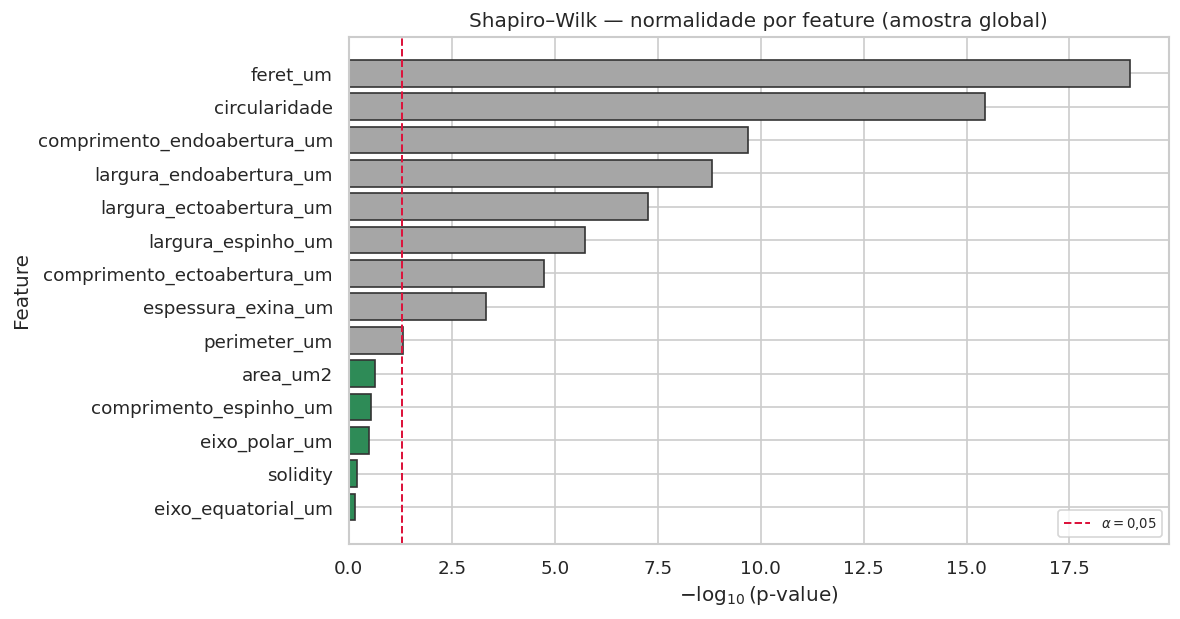
\includegraphics[width=0.85\textwidth]{shapiro_wilk_significancia.png}
\caption{Resultados do teste de Shapiro--Wilk por \textit{feature} ($\alpha = 0{,}05$; $n = 89$ grãos imputados).}\label{fig:shapiro}
\end{figure}

\begin{figure}[H]
\centering
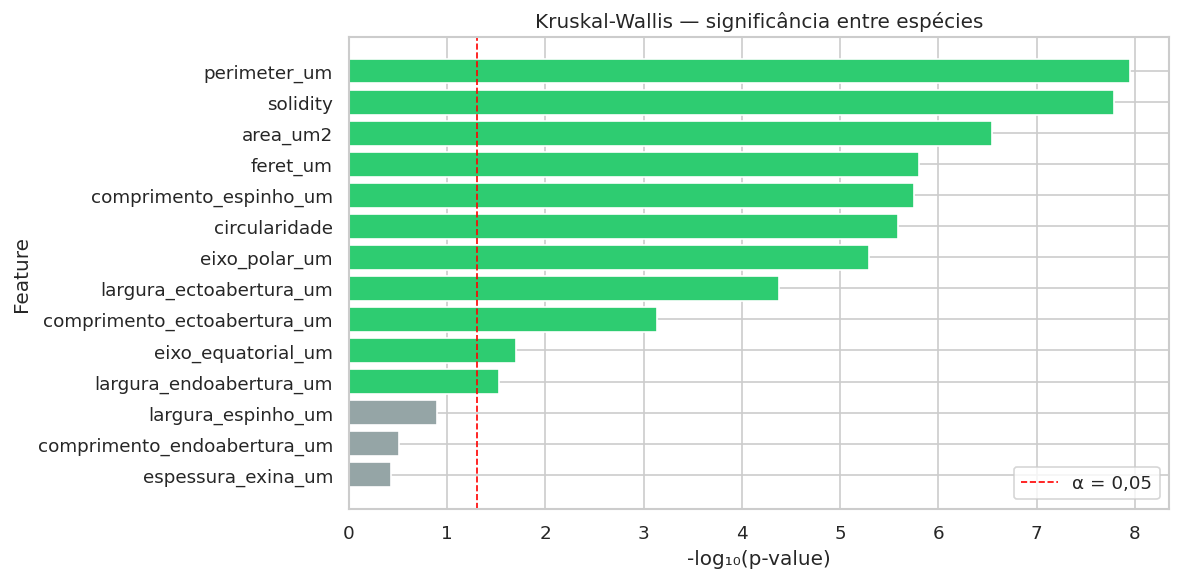
\includegraphics[width=0.85\textwidth]{kruskal_wallis_significancia.png}
\caption{Significância estatística das diferenças entre espécies (Kruskal--Wallis, $\alpha = 0{,}05$) para 14 traits morfométricas.}\label{fig:kruskal}
\end{figure}

\paragraph{Correlação entre variáveis.} A matriz de correlação de Pearson (Fig.~\ref{fig:correlacao}) evidenciou forte associação linear entre medidas de tamanho global --- área, perímetro e Feret ($|r| > 0{,}70$) ---, indicando redundância parcial entre \textit{features} morfométricas e reforçando a necessidade de abordagens multivariadas para discriminação taxonômica.

\begin{figure}[H]
\centering
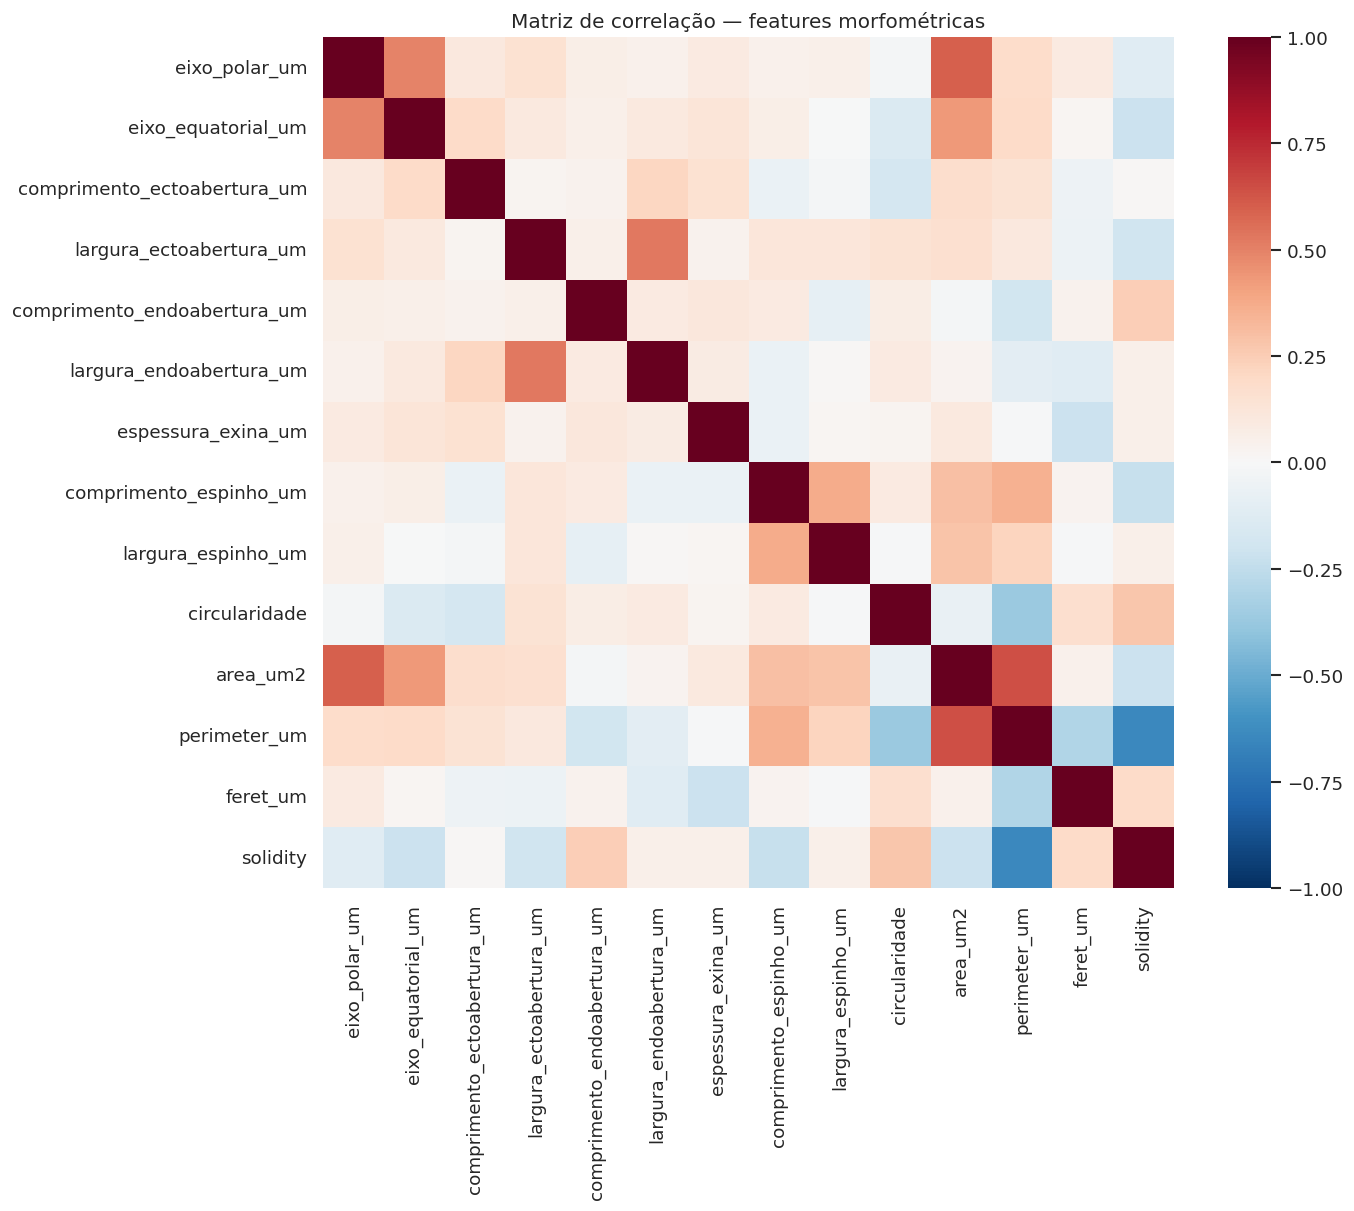
\includegraphics[width=0.85\textwidth]{correlacao_features.png}
\caption{Matriz de correlação de Pearson entre as 14 \textit{features} morfométricas (dados imputados).}\label{fig:correlacao}
\end{figure}

\paragraph{Análise de componentes principais (PCA).} A PCA sobre as 14 variáveis padronizadas (\textit{z-score}) indicou que os dois primeiros componentes explicam, respectivamente, 21,0\% e 13,1\% da variância total (34,1\% acumulados; Fig.~\ref{fig:scree}). No plano PC1--PC2 (Fig.~\ref{fig:pca}), \textit{C. hatschbachii} ocupa região parcialmente segregada das demais espécies (elipses de confiança $\approx$95\%), ao passo que \textit{C. longiangustatus}, \textit{C. rupestris} e \textit{C. ruschianus} apresentam elipses amplamente sobrepostas. Os \textit{loadings} (Fig.~\ref{fig:loadings}) indicam que solidez, área, perímetro e comprimento do espinho contribuem fortemente para PC1, enquanto eixo polar e largura da ectoabertura influenciam PC2.

\begin{figure}[H]
\centering
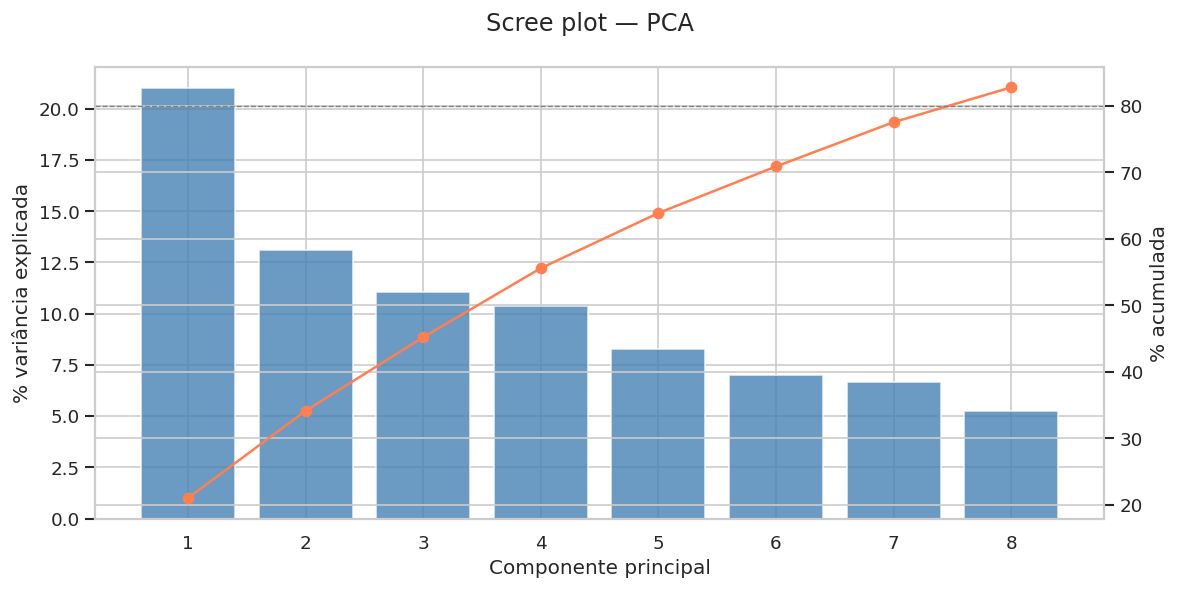
\includegraphics[width=0.75\textwidth]{pca_scree.png}
\caption{Scree plot da PCA: variância explicada por cada componente principal.}\label{fig:scree}
\end{figure}

\begin{figure}[H]
\centering
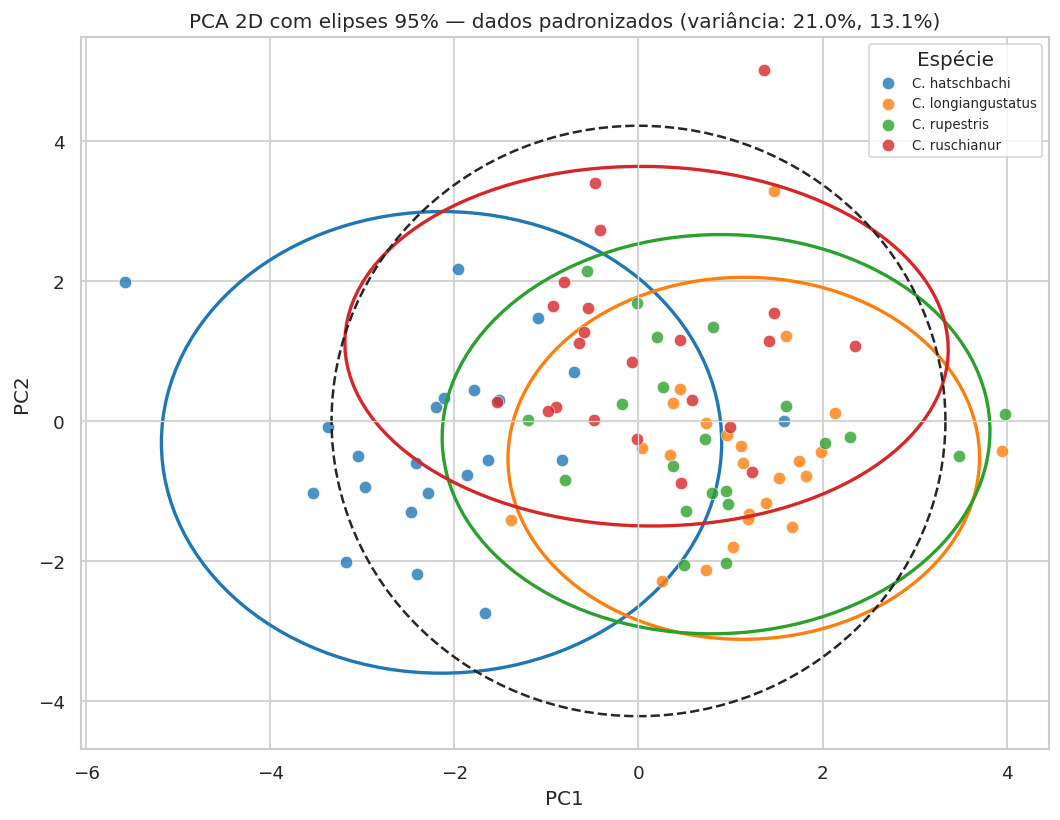
\includegraphics[width=0.85\textwidth]{pca_especies_elipse.png}
\caption{PCA 2D (PC1 \textit{vs.} PC2) com elipses de confiança $\approx$95\% por espécie (dados padronizados).}\label{fig:pca}
\end{figure}

\begin{figure}[H]
\centering
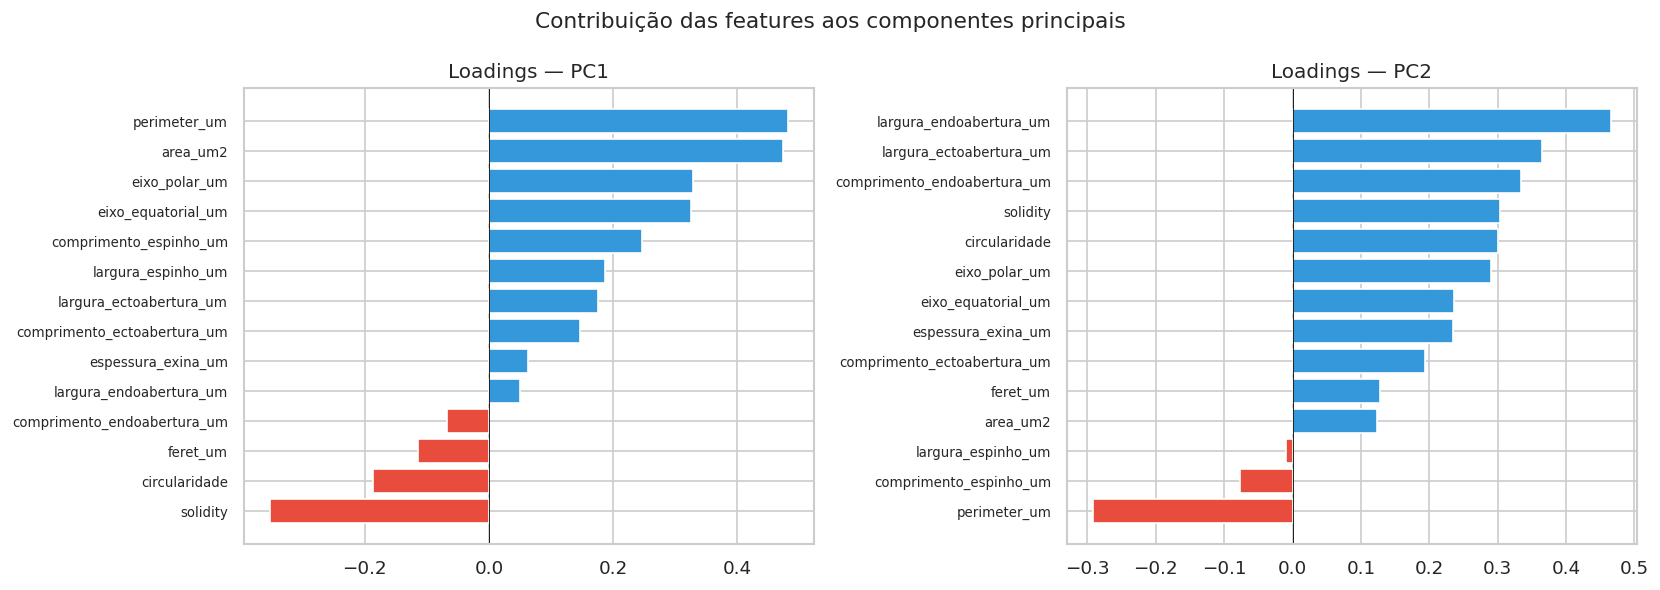
\includegraphics[width=0.85\textwidth]{pca_loadings.png}
\caption{Contribuição (\textit{loadings}) das \textit{features} nos dois primeiros componentes principais.}\label{fig:loadings}
\end{figure}

\paragraph{Relações bivariadas e perfil morfométrico.} A relação entre eixos polar e equatorial (Fig.~\ref{fig:eixos}) confirma concentração na faixa de 30--35~$\mu$m (polar) e 32--37~$\mu$m (equatorial), com mistura entre \textit{C. longiangustatus}, \textit{C. rupestris} e \textit{C. ruschianus}. \textit{C. hatschbachii} inclui grãos com eixo polar menor ($\approx$25--29~$\mu$m), parcialmente afastados do núcleo comum. As aberturas (Fig.~\ref{fig:aberturas}) mostram que \textit{C. rupestris} tende a valores mais altos de largura da ectoabertura ($\approx$6--10~$\mu$m), enquanto \textit{C. hatschbachii} concentra-se em larguras menores ($\approx$3--5~$\mu$m). Os scatter plots bivariados (Fig.~\ref{fig:morfologia}) indicam que a combinação área + perímetro + solidez é a mais promissora para separar \textit{C. hatschbachii} das demais espécies. O heatmap de perfil por espécie (Fig.~\ref{fig:perfil}), com médias padronizadas, resume visualmente essas diferenças relativas entre táxons.

\begin{figure}[H]
\centering
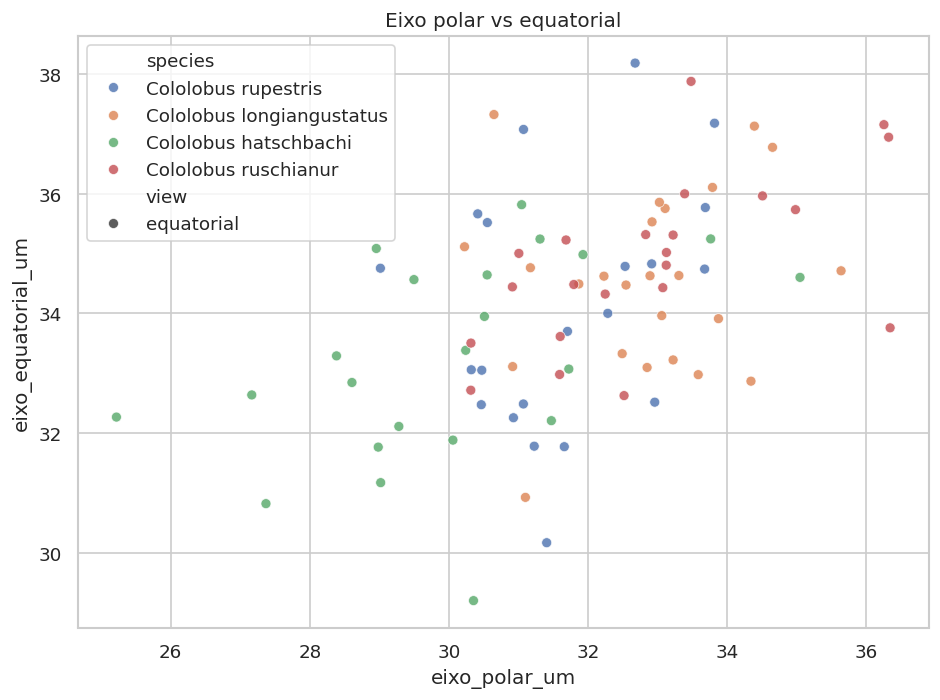
\includegraphics[width=0.75\textwidth]{scatter_eixos.png}
\caption{Relação entre eixo polar e eixo equatorial ($\mu$m) por espécie.}\label{fig:eixos}
\end{figure}

\begin{figure}[H]
\centering
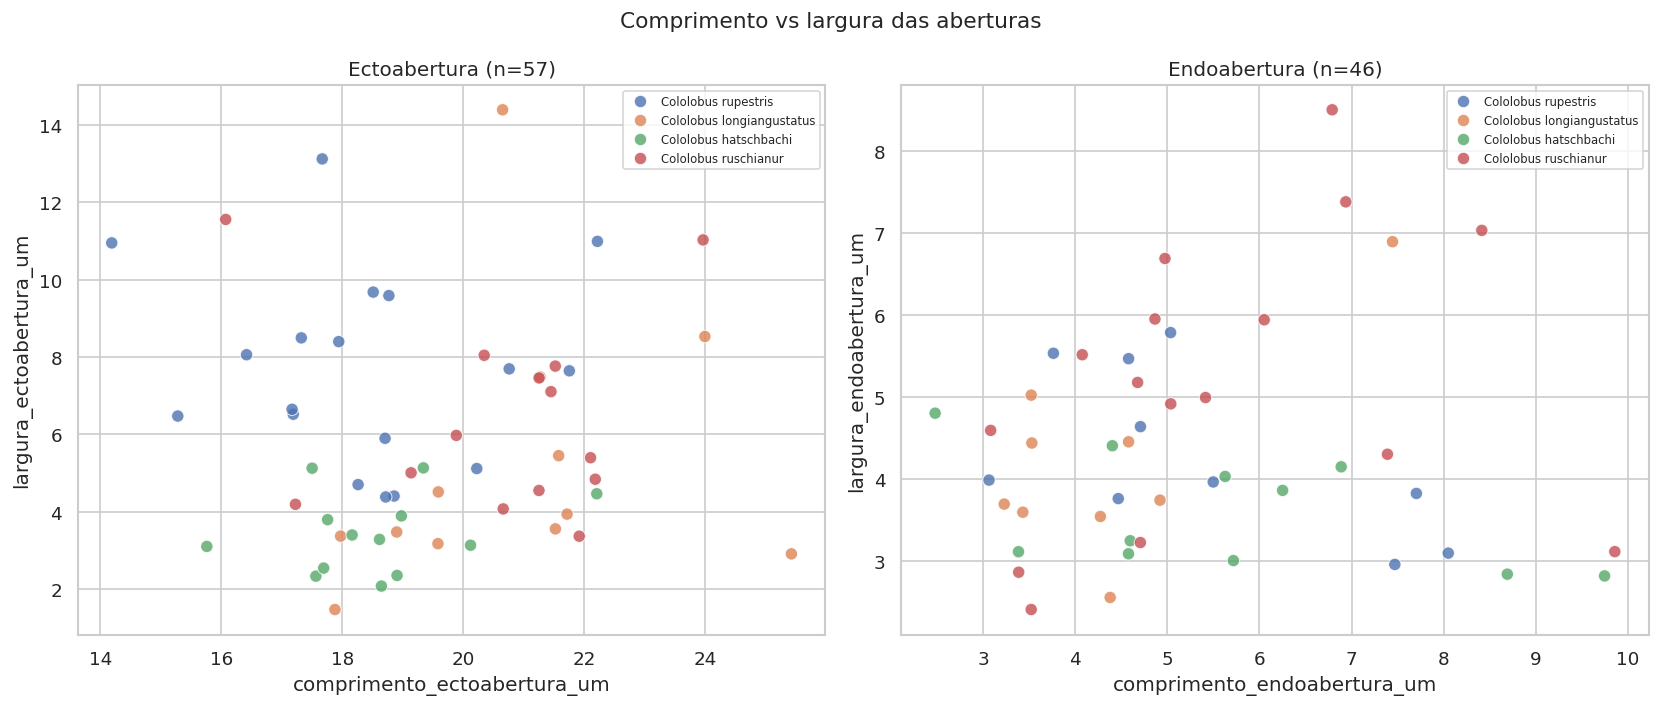
\includegraphics[width=0.85\textwidth]{scatter_aberturas.png}
\caption{Relação entre comprimento e largura das ectoaberturas (esquerda; $n = 57$) e endoaberturas (direita; $n = 46$).}\label{fig:aberturas}
\end{figure}

\begin{figure}[H]
\centering
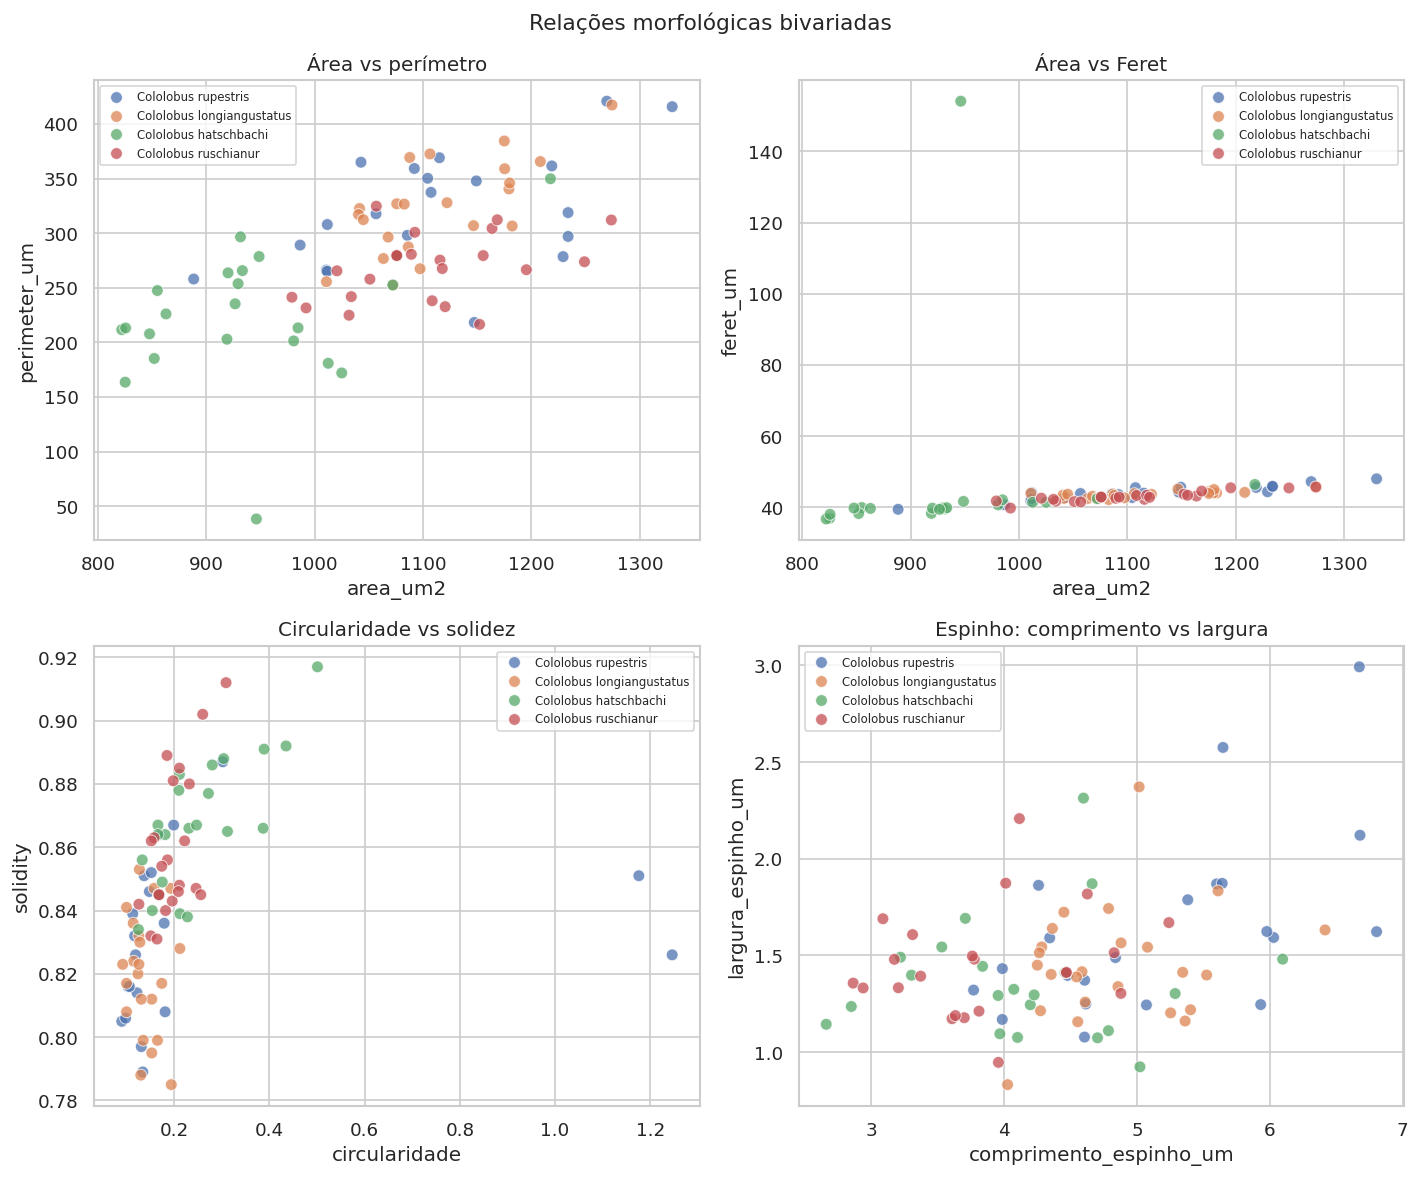
\includegraphics[width=0.98\textwidth,height=0.9\textheight,keepaspectratio]{scatter_morfologia.png}
\caption{Relações morfológicas bivariadas: área \textit{vs.} perímetro; área \textit{vs.} Feret; circularidade \textit{vs.} solidez; comprimento \textit{vs.} largura do espinho.}\label{fig:morfologia}
\end{figure}

\begin{figure}[H]
\centering
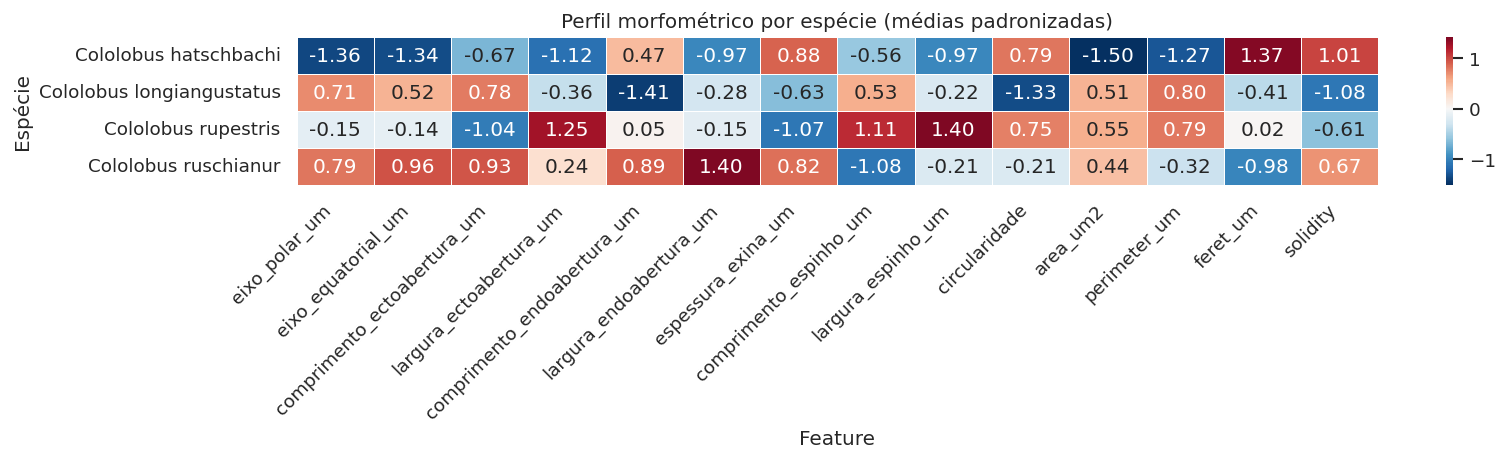
\includegraphics[width=0.85\textwidth]{heatmap_perfil_especies.png}
\caption{Perfil morfométrico por espécie: médias padronizadas (\textit{z-score}) das 14 \textit{features}.}\label{fig:perfil}
\end{figure}

\FloatBarrier
\subsection{Classificação supervisionada de espécies}\label{subsec:ml}

A necessidade de abordagens multivariadas indicada pela análise exploratória, sobreposição no PCA, correlação entre medidas de tamanho e mistura nos scatter plots, foi endereçada por classificação supervisionada. Para evitar vazamento de dados, a imputação de medianas e a padronização (\textit{z-score}) foram encapsuladas em um \textit{pipeline} ajustado independentemente em cada \textit{fold} da validação cruzada. Após o ajuste de hiperparâmetros por busca em grade, o modelo SVM com \textit{kernel} RBF ($C = 1$, $\gamma = 0{,}1$) obteve o melhor desempenho, com F1-macro de $0{,}716 \pm 0{,}140$ na validação cruzada estratificada, praticamente empatado com o Random Forest ($0{,}715 \pm 0{,}065$); ambos superaram amplamente a linha de base aleatória ($0{,}209$), confirmando que a morfometria carrega sinal taxonômico substancial (Tab.~\ref{tab:ml_modelos}; Fig.~\ref{fig:ml_comp}). O modelo final atingiu acurácia global de $0{,}72$.

% Tabelas de resultados do aprendizado de máquina.
% Inclua no relatório com: % Tabelas de resultados do aprendizado de máquina.
% Inclua no relatório com: % Tabelas de resultados do aprendizado de máquina.
% Inclua no relatório com: \input{tabela_ml_resultados.tex}
% Requer no preâmbulo: \usepackage{booktabs}

\begin{table}[htbp]
\caption{Comparação dos modelos de classificação por validação cruzada estratificada (5-\textit{fold}). Métricas: média $\pm$ desvio-padrão entre \textit{folds}.}\label{tab:ml_modelos}
\begin{tabular*}{\textwidth}{@{\extracolsep\fill}lcc@{}}
\toprule
Modelo & F1-macro & Acurácia \\
\midrule
\textit{Dummy} (linha de base) & $0{,}209 \pm 0{,}028$ & $0{,}202 \pm 0{,}025$ \\
Random Forest                  & $0{,}715 \pm 0{,}065$ & $0{,}719 \pm 0{,}061$ \\
SVM (kernel RBF)               & $\mathbf{0{,}716} \pm 0{,}140$ & $\mathbf{0{,}719} \pm 0{,}145$ \\
\botrule
\end{tabular*}
\footnotetext{Modelo final: SVM RBF, selecionado pelo maior F1-macro. A imputação (mediana) e a padronização (\textit{z-score}) foram ajustadas dentro de cada \textit{fold} da validação cruzada, evitando vazamento de dados. Hiperparâmetros otimizados por \texttt{GridSearchCV}: SVM ($C=1$, $\gamma=0{,}1$); Random Forest (\texttt{n\_estimators}$=100$, \texttt{max\_depth}$=$None, \texttt{max\_features}$=$sqrt, \texttt{min\_samples\_leaf}$=2$).}
\end{table}

\begin{table}[htbp]
\caption{Desempenho por espécie do modelo final (SVM RBF), com predições \textit{out-of-fold}.}\label{tab:ml_classes}
\begin{tabular*}{\textwidth}{@{\extracolsep\fill}lcccc@{}}
\toprule
Espécie & Precisão & \textit{Recall} & F1 & Suporte \\
\midrule
\textit{C. hatschbachii}    & 0{,}905 & 0{,}864 & 0{,}884 & 22 \\
\textit{C. longiangustatus} & 0{,}621 & 0{,}750 & 0{,}679 & 24 \\
\textit{C. rupestris}       & 0{,}591 & 0{,}619 & 0{,}605 & 21 \\
\textit{C. ruschianus}      & 0{,}824 & 0{,}636 & 0{,}718 & 22 \\
\botrule
\end{tabular*}
\footnotetext{Acurácia global $= 0{,}719$; F1-macro $= 0{,}721$. Clusterização exploratória (K-Means, $k=4$): \textit{Adjusted Rand Index} (ARI) $= 0{,}233$.}
\end{table}

% Requer no preâmbulo: \usepackage{booktabs}

\begin{table}[htbp]
\caption{Comparação dos modelos de classificação por validação cruzada estratificada (5-\textit{fold}). Métricas: média $\pm$ desvio-padrão entre \textit{folds}.}\label{tab:ml_modelos}
\begin{tabular*}{\textwidth}{@{\extracolsep\fill}lcc@{}}
\toprule
Modelo & F1-macro & Acurácia \\
\midrule
\textit{Dummy} (linha de base) & $0{,}209 \pm 0{,}028$ & $0{,}202 \pm 0{,}025$ \\
Random Forest                  & $0{,}715 \pm 0{,}065$ & $0{,}719 \pm 0{,}061$ \\
SVM (kernel RBF)               & $\mathbf{0{,}716} \pm 0{,}140$ & $\mathbf{0{,}719} \pm 0{,}145$ \\
\botrule
\end{tabular*}
\footnotetext{Modelo final: SVM RBF, selecionado pelo maior F1-macro. A imputação (mediana) e a padronização (\textit{z-score}) foram ajustadas dentro de cada \textit{fold} da validação cruzada, evitando vazamento de dados. Hiperparâmetros otimizados por \texttt{GridSearchCV}: SVM ($C=1$, $\gamma=0{,}1$); Random Forest (\texttt{n\_estimators}$=100$, \texttt{max\_depth}$=$None, \texttt{max\_features}$=$sqrt, \texttt{min\_samples\_leaf}$=2$).}
\end{table}

\begin{table}[htbp]
\caption{Desempenho por espécie do modelo final (SVM RBF), com predições \textit{out-of-fold}.}\label{tab:ml_classes}
\begin{tabular*}{\textwidth}{@{\extracolsep\fill}lcccc@{}}
\toprule
Espécie & Precisão & \textit{Recall} & F1 & Suporte \\
\midrule
\textit{C. hatschbachii}    & 0{,}905 & 0{,}864 & 0{,}884 & 22 \\
\textit{C. longiangustatus} & 0{,}621 & 0{,}750 & 0{,}679 & 24 \\
\textit{C. rupestris}       & 0{,}591 & 0{,}619 & 0{,}605 & 21 \\
\textit{C. ruschianus}      & 0{,}824 & 0{,}636 & 0{,}718 & 22 \\
\botrule
\end{tabular*}
\footnotetext{Acurácia global $= 0{,}719$; F1-macro $= 0{,}721$. Clusterização exploratória (K-Means, $k=4$): \textit{Adjusted Rand Index} (ARI) $= 0{,}233$.}
\end{table}

% Requer no preâmbulo: \usepackage{booktabs}

\begin{table}[htbp]
\caption{Comparação dos modelos de classificação por validação cruzada estratificada (5-\textit{fold}). Métricas: média $\pm$ desvio-padrão entre \textit{folds}.}\label{tab:ml_modelos}
\begin{tabular*}{\textwidth}{@{\extracolsep\fill}lcc@{}}
\toprule
Modelo & F1-macro & Acurácia \\
\midrule
\textit{Dummy} (linha de base) & $0{,}209 \pm 0{,}028$ & $0{,}202 \pm 0{,}025$ \\
Random Forest                  & $0{,}715 \pm 0{,}065$ & $0{,}719 \pm 0{,}061$ \\
SVM (kernel RBF)               & $\mathbf{0{,}716} \pm 0{,}140$ & $\mathbf{0{,}719} \pm 0{,}145$ \\
\botrule
\end{tabular*}
\footnotetext{Modelo final: SVM RBF, selecionado pelo maior F1-macro. A imputação (mediana) e a padronização (\textit{z-score}) foram ajustadas dentro de cada \textit{fold} da validação cruzada, evitando vazamento de dados. Hiperparâmetros otimizados por \texttt{GridSearchCV}: SVM ($C=1$, $\gamma=0{,}1$); Random Forest (\texttt{n\_estimators}$=100$, \texttt{max\_depth}$=$None, \texttt{max\_features}$=$sqrt, \texttt{min\_samples\_leaf}$=2$).}
\end{table}

\begin{table}[htbp]
\caption{Desempenho por espécie do modelo final (SVM RBF), com predições \textit{out-of-fold}.}\label{tab:ml_classes}
\begin{tabular*}{\textwidth}{@{\extracolsep\fill}lcccc@{}}
\toprule
Espécie & Precisão & \textit{Recall} & F1 & Suporte \\
\midrule
\textit{C. hatschbachii}    & 0{,}905 & 0{,}864 & 0{,}884 & 22 \\
\textit{C. longiangustatus} & 0{,}621 & 0{,}750 & 0{,}679 & 24 \\
\textit{C. rupestris}       & 0{,}591 & 0{,}619 & 0{,}605 & 21 \\
\textit{C. ruschianus}      & 0{,}824 & 0{,}636 & 0{,}718 & 22 \\
\botrule
\end{tabular*}
\footnotetext{Acurácia global $= 0{,}719$; F1-macro $= 0{,}721$. Clusterização exploratória (K-Means, $k=4$): \textit{Adjusted Rand Index} (ARI) $= 0{,}233$.}
\end{table}


\begin{figure}[H]
\centering
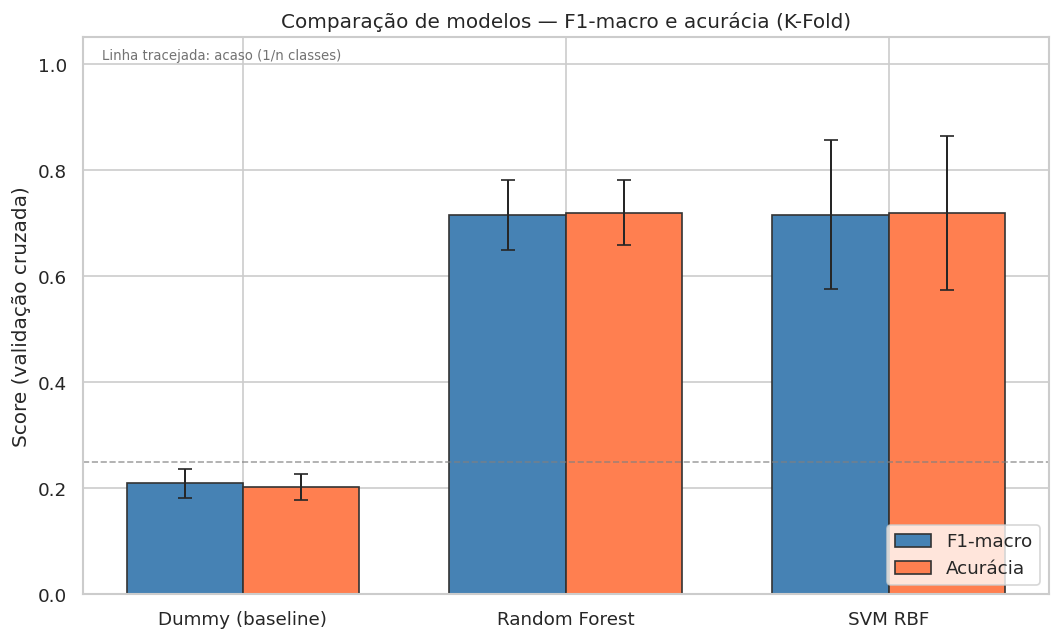
\includegraphics[width=0.85\textwidth]{ml_comparacao_metricas.png}
\caption{Comparação de F1-macro e acurácia entre os modelos avaliados na validação cruzada de cinco \textit{folds}.}\label{fig:ml_comp}
\end{figure}

O desempenho por espécie (Tab.~\ref{tab:ml_classes}) mostra que \textit{C. hatschbachii} é a classe mais bem identificada (F1 $= 0{,}88$), enquanto \textit{C. rupestris} apresenta o menor F1 ($0{,}61$). A matriz de confusão (Fig.~\ref{fig:ml_cm}) evidencia que os erros concentram-se entre \textit{C. longiangustatus}, \textit{C. rupestris} e \textit{C. ruschianus}, sendo o par \textit{C. rupestris} $\leftrightarrow$ \textit{C. longiangustatus} o mais confundido. A análise de importância por permutação (Tab.~\ref{tab:features}; Fig.~\ref{fig:ml_imp}) apontou comprimento do espinho, eixo polar, solidez e largura da ectoabertura como as variáveis mais relevantes para a discriminação --- em consonância com as \textit{traits} mais significativas no teste de Kruskal-Wallis. Por fim, a clusterização não supervisionada por K-Means recuperou apenas fracamente a estrutura de espécies (ARI $= 0{,}23$), reforçando que os táxons não formam agrupamentos naturais bem separados no espaço morfométrico e que a separação exige aprendizado supervisionado.

\begin{figure}[H]
\centering
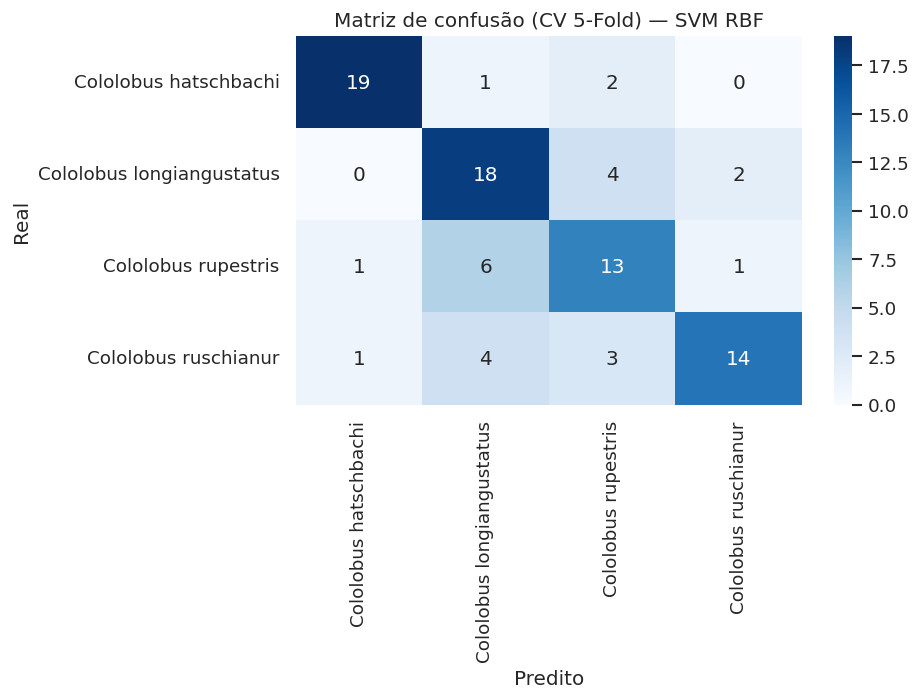
\includegraphics[width=0.7\textwidth]{confusion_matrix.png}
\caption{Matriz de confusão do modelo final (SVM RBF) com predições \textit{out-of-fold} na validação cruzada de cinco \textit{folds}.}\label{fig:ml_cm}
\end{figure}

\begin{figure}[H]
\centering
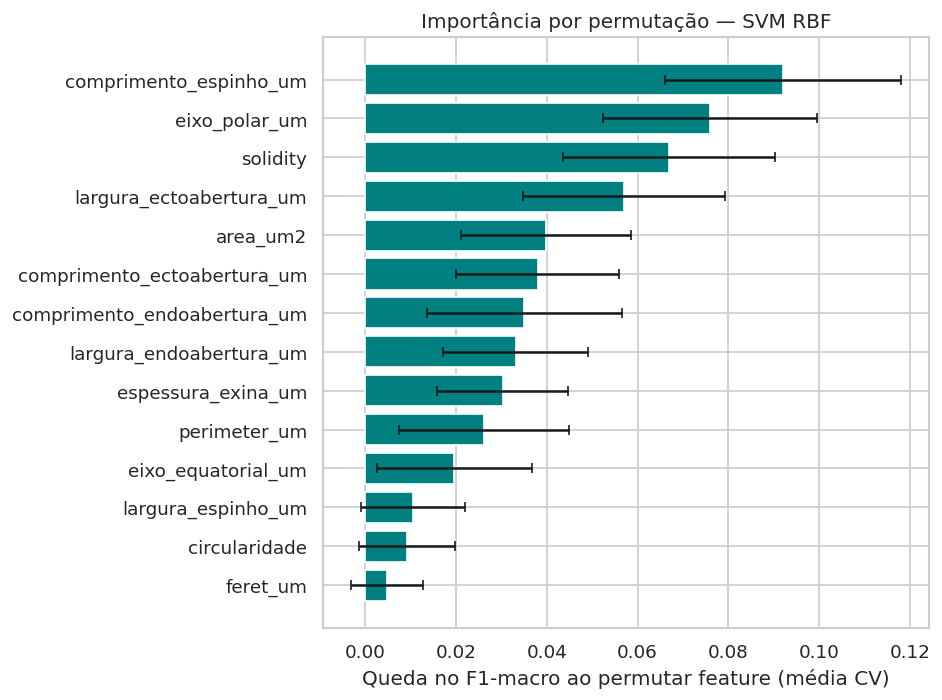
\includegraphics[width=0.85\textwidth]{ml_permutation_importance.png}
\caption{Importância das variáveis por permutação no modelo final (queda média em F1-macro ao permutar cada \textit{feature}).}\label{fig:ml_imp}
\end{figure}

\FloatBarrier
%%======================================================================
\section{Discussão}\label{sec:discussao}
%%======================================================================

A análise micromorfológica de quatro espécies de \textit{Cololobus} aponta que os grãos de pólen são médios, isopolares, oblato-esferoidais, tricolporados, subequinolofados e com teto microperfurado, evidenciando a conservação desses caracteres entre as espécies. O comprimento dos espinhos, por sua vez, é um caráter mais informativo para a delimitação em nível específico. Semelhantemente, Siniscalchi et al. \cite{siniscalchi2017} e Vega e Dematteis \cite{vega2011} consideraram o tamanho dos espinhos um caráter relevante para delimitação de espécies de \textit{Chresta} e \textit{Vernonanthura}.

Os grãos de pólen das espécies analisadas caracterizam-se no tipo~A por serem tricolporados, subequinolofados e possuírem o teto continuamente microperfurado \cite{keeley1977,keeley1979}. Entre os seis tipos de pólen descritos para espécies de \textit{Vernonia}, o tipo~A é o mais frequente, distribuído mundialmente \cite{keeley1979}. Ademais, esse mesmo tipo de pólen pode ser encontrado em outros gêneros da tribo Vernonieae, como \textit{Chresta} \cite{siniscalchi2017}, \textit{Eremanthus} \cite{loeuille2012}, \textit{Paralychnophora} \cite{souzasouza2016}, \textit{Piptolepis} \cite{souzasouza2022} e \textit{Vernonanthura} \cite{vega2011}.

Esse conjunto de caracteres parece representar um padrão conservado dentro de subtribos como Vernoniinae e Lychnophorinae, onde o tipo~A é mais frequente \cite{dematteis2008,vega2011,souzasouza2016,siniscalchi2017,souzasouza2022}. Em Lepidaploinae, por sua vez, outros tipos de pólen, como B, C e G, são amplamente encontrados entre as espécies \cite{angulo2010,marques2021}.

O formato oblato-esferoidal, descrito para todas as espécies de \textit{Cololobus}, não é o mais recorrente em outros gêneros da subtribo Vernoniinae \cite{dematteis2008,vega2011}. Em espécies de \textit{Vernonia} e \textit{Vernonanthura}, o formato mais comum de pólen é o prolato-esferoidal; em contrapartida, o formato oblato-esferoidal foi observado apenas em \textit{Vernonia hassleriana}, \textit{V. hystrix}, \textit{V. lipeoensis}, \textit{V. propinqua} e \textit{V. schulziana} \cite{dematteis2008,vega2011}. Assim, a forma dos grãos de pólen pode apresentar variações entre gêneros, constituindo um caráter potencialmente informativo em nível genérico.

A análise exploratória morfométrica de 89 grãos em vista equatorial complementa a descrição qualitativa ao demonstrar que as espécies estudadas não são morfometricamente idênticas: 11 das 14 variáveis testadas apresentaram diferenças significativas pelo teste de Kruskal--Wallis ($\alpha = 0{,}05$; Tab.~\ref{tab:features}; Fig.~\ref{fig:kruskal}). A PCA (Fig.~\ref{fig:pca}) confirma parcial segregação de \textit{C. hatschbachii} no plano PC1--PC2, enquanto as demais espécies permanecem sobrepostas. Entretanto, a significância estatística não implica separação completa entre táxons, pois os violin plots, scatter plots e elipses de confiança revelam ampla sobreposição distribucional (Figs.~\ref{fig:violinos}--\ref{fig:morfologia}), sobretudo entre \textit{C. longiangustatus}, \textit{C. rupestris} e \textit{C. ruschianus}. Esse padrão indica que a delimitação específica em \textit{Cololobus} provavelmente depende da combinação de múltiplos caracteres, relacionados ao tamanho global, à forma e à ornamentação da exina, e não de uma única medida isolada, como já observado em outros gêneros morfologicamente conservados da Vernonieae.

Os resultados do aprendizado de máquina quantificam essa separabilidade multivariada. O F1-macro de $0{,}72$ obtido pelo SVM RBF, muito superior à linha de base aleatória, demonstra que o conjunto das 14 \textit{features} carrega sinal taxonômico suficiente para discriminar automaticamente a maioria dos grãos. O desempenho praticamente equivalente entre SVM RBF e Random Forest ($0{,}716$ \textit{vs.} $0{,}715$ de F1-macro) indica que o sinal discriminante é robusto e não depende de um único tipo de modelo, sendo capturado tanto por fronteiras de decisão não lineares (SVM) quanto por ensembles de árvores (RF). O padrão de acertos e erros do classificador reproduz fielmente a estrutura observada na análise exploratória: \textit{C. hatschbachii}, a espécie morfologicamente mais distinta, foi a mais bem classificada (F1 $= 0{,}88$), ao passo que \textit{C. longiangustatus}, \textit{C. rupestris} e \textit{C. ruschianus} concentraram os erros de confusão mútua (Tab.~\ref{tab:ml_classes}; Fig.~\ref{fig:ml_cm}). O baixo \textit{Adjusted Rand Index} do K-Means (ARI $= 0{,}23$) confirma que, sem supervisão, os táxons não emergem como agrupamentos naturais bem definidos, indicando limites morfométricos tênues entre as espécies congêneres. Do ponto de vista sistemático, as variáveis de maior importância no classificador --- comprimento do espinho, eixo polar e solidez --- convergem com as \textit{traits} mais significativas na estatística univariada, reforçando quais caracteres devem ser priorizados em futuras chaves de identificação.

Qualitativamente, os espinhos são mais longos em \textit{C. hatschbachii} e \textit{C. longiangustatus} e tendem a ser mais curtos em \textit{C. rupestris} e \textit{C. ruschianus} (Fig.~\ref{fig:prancha}; Tab.~\ref{tab:medidas}). Na morfometria, o comprimento do espinho foi uma das variáveis mais discriminantes tanto no Kruskal-Wallis quanto na importância por permutação do classificador, ao passo que a largura do espinho não apresentou diferença significativa entre espécies. Os scatter plots de comprimento versus largura do espinho (Fig.~\ref{fig:morfologia}) mostram considerável dispersão intra e interespecífica, com sobreposição entre \textit{C. longiangustatus}, \textit{C. rupestris} e \textit{C. ruschianus}. Portanto, o tamanho dos espinhos, especialmente o comprimento, permanece informativo para a delimitação específica, mas deve ser interpretado em conjunto com outras traits e com cautela quanto à variabilidade individual dos grãos.

A morfometria das aberturas fornece evidência discriminativa parcial. A largura da ectoabertura tende a ser maior em \textit{C. rupestris} ($\approx$6--10~$\mu$m) e menor em \textit{C. hatschbachii} ($\approx$3--5~$\mu$m), enquanto \textit{C. longiangustatus} e \textit{C. ruschianus} ocupam a região central com forte mistura (Fig.~\ref{fig:aberturas}). A endoabertura apresenta sobreposição ainda maior entre as quatro espécies, o que é coerente com a não significância estatística do comprimento da endoabertura no Kruskal-Wallis. Ressalta-se que 34--48\% dos registros não possuem medidas de abertura, o que reduz o poder estatístico e pode subestimar o valor diagnóstico desses caracteres, os quais, na descrição qualitativa (endoabertura lalongada com constrição mediana; Fig.~\ref{fig:prancha}), permanecem relevantes morfologicamente, embora sejam difíceis de quantificar de forma consistente em vista equatorial.

Variáveis relacionadas ao tamanho global do grão (área, perímetro e Feret) e à forma (solidez e circularidade) concentraram-se entre as mais significativas no Kruskal-Wallis (Tab.~\ref{tab:features}). A solidez, em particular, contribui para separar \textit{C. hatschbachii} das demais espécies, enquanto a circularidade exibiu caudas longas e valores atípicos em alguns táxons, possivelmente em função de variabilidade intraespecífica, da orientação do grão na medição ou de grãos morfologicamente aberrantes. Em contraste, a espessura da exina, descrita qualitativamente como mais delgada em \textit{C. rupestris} (Tab.~\ref{tab:medidas}), não diferiu significativamente entre espécies na análise exploratória, indicando que esse caráter, embora útil na descrição micromorfológica, possui baixo poder discriminatório no conjunto amostral analisado.

Em conjunto, os resultados micromorfológicos, morfométricos e de aprendizado de máquina ampliam o conhecimento palinológico de \textit{Cololobus} e indicam que o gênero exibe uma morfologia polínica conservada (tipo~A, tricolporado, subequinolofado) com variação quantitativa detectável principalmente em tamanho, forma e comprimento dos espinhos. A delimitação de \textit{C. hatschbachii} é a mais robusta, sendo consistentemente separada tanto na estatística univariada quanto pelo classificador; entre as demais espécies, a morfometria equatorial sugere limites taxonômicos menos nítidos. Como limitações, destacam-se o tamanho amostral reduzido (cerca de 22 grãos por espécie), que restringe a generalização e o ajuste fino dos modelos, e a elevada proporção de dados ausentes nas medidas de abertura. Estudos futuros poderiam incorporar mais grãos e vistas polares, ampliar a amostragem de aberturas, quantificar densidade e espaçamento dos espinhos e combinar dados palinológicos com evidências moleculares para testar hipóteses de delimitação específica no gênero.

\backmatter

\bmhead{Agradecimentos ao professor Dr. Leandro Nogueira Couto pelos ensinamentos durante a disciplina Mineração de Dados e ao professor Dr. Danilo Marques pela disponibilização do material para realização do estudo}



\bibliography{cololobus-bibliography}

\end{document}
